\documentclass[pra,twocolumn,superscriptaddress,floatfix,nofootinbib,amsmath,amssymb]{revtex4-1}

\usepackage[english]{babel}
\usepackage[T1]{fontenc}
\usepackage{xeCJK}
\usepackage{float}
\usepackage{graphicx}
\usepackage{bm}
\usepackage{braket}
\usepackage{xcolor}
\usepackage{amsfonts}
\usepackage{comment}
\usepackage{dirtytalk}
\usepackage[hidelinks]{hyperref}
\usepackage{cleveref}
\usepackage{url}
\usepackage{bbold}
\usepackage{realboxes}
\usepackage{my_macro}
\usepackage{enumitem}
\usepackage{booktabs}
\usepackage{algpseudocode}

\newcommand{\fancylink}[2]{\[\footnotesize\Colorbox{bkgd}{\color{orange-red}\href{#1}{\linkcode{#2}}}\]}

\newcommand{\spliteq}[1]{\begin{equation}
\begin{split}
#1
\end{split}
\end{equation}
}

\newcommand{\tr}{\text{tr}}

\usepackage{listings}
\usepackage{xcolor}

\UseRawInputEncoding
\usepackage{titlesec} %自定义多级标题格式的宏包
\titleformat{\paragraph}[block]{\small\bfseries}{}{}{}[]
% \titleformat{\paragraph}[block]{\small\bfseries}{}{1em}{}[]

\definecolor{bkgd}{RGB}{240,242,246}
\definecolor{ceruleanblue}{rgb}{0.16, 0.32, 0.75}
\definecolor{orange-red}{rgb}{1.0, 0.27, 0.0}
\definecolor{anotherblue}{RGB}{37,92,243}
\definecolor{blackblue}{RGB}{46,60,85}
\definecolor{goldyellow}{RGB}{199,146,12}
\lstdefinestyle{altstyle2}{
    backgroundcolor=\color{bkgd},
    basicstyle=\ttfamily\footnotesize\color{blackblue},
    breakatwhitespace=false,
    breaklines=true,
    captionpos=b,
    commentstyle=\color{goldyellow},
    keepspaces=true,
    keywordstyle=\color{orange-red},
    language=Python,
    numbersep=5pt,
    numberstyle=\tiny\color{ceruleanblue},
    showspaces=false,
    showstringspaces=false,
    showtabs=false,
    stringstyle=\color{anotherblue},
    tabsize=2
}
\lstset{style=altstyle2}

\bibliographystyle{apsrev4-1}

\begin{document}

\title{MindSpore Quantum: XXXXXXXXX
}


\affiliation{HuaWei
}

\author{author}
\email{email}

\affiliation{organization
}

\date{\today}

\keywords{quantum machine learning, neural networks, quantum neural networks, variational quantum algorithms, machine learning, quantum algorithms}


\begin{abstract}
    Abstract
\end{abstract}
\maketitle
\tableofcontents

\section{Introduction}
Introduction of MindSpore Quantum.
\input{1_Introduction}

\section{Elements of MindSpore Quantum}

\subsection{Data Type}
View demo code of this section: \democode{02}{2.1}

In this section, we will introduce the basic data types supported by \MindQuantum. When we simulate quantum evolution in \MindQuantum, different data types require different sizes of computer memory and lead to different simulation accuracy.
Before we discuss the supported data types in \MindQuantum, we first briefly review the definition of the floating-point number in modern computers which helps us to understand the difference among these data types.
The first unified technical standard of floating-point arithmetic (IEEE 754) was established in 1985 and is widely supported by much hardware today by the Institute of Electrical and Electronics Engineers (IEEE).

% TODO(xusheng): Add figure
In IEEE 754, a floating-point format is specified by three parts, sign, exponent, and fraction, all of which consist of a ${0,1}$ bit string as shown in Fig.

The sign bit $s$ determines the sign of the number, $s=0$ is positive and $s=1$ is negative.
The exponent part $e$ is an m-bit unsigned integer, which determines the Maximum and minimum values, and the fraction part $\vec{b}$ with $n$ bits is the true significance that appears in the memory format which determines the precision of the number.

The real value assumed by a given sign $s$, biased exponent $e$ and fraction $\vec{b}$ as
\begin{equation}
    value = (-1)^{s}\times 2^{e}\times (1+\sum_{i=1}^nb_{23-i}2^{-i})
\end{equation}

Based on the different numbers of bits, IEEE 754 defined three types of floating-point formats single-, double- and quadruple-precision with 32, 64, and 128 bits, respectively.
Among them, single- and double-precision is widely used in classical computers.
In single-precision floating-point format (for short, denoted as Single as follow), sign $s$ consists of $1$ bit, $8$ bits in the exponent part $e$, and $23$ bits in the fraction part $\vec{b}$.
In double-precision floating-point format (Double), sign $s$ still consists of $1$ bit, $11$ bits in the exponent part $e$, and $52$ bits in the fraction part $\vec{b}$.

The value precision is determined by the number of bits in the fraction part.
In Single, the fraction part is $\vec{b}=0.b_{22}b_{21}\cdots b{0}$.
In fact, the first $0$ is default as $1$, so the true fraction part is $1.b_{22}b_{21}\cdots b{0}$, that can explain the Eq.() where $\vec{b}$ plus $1$.
Then the total precision of Single is 24 bits which approximates $7.22$ decimal digits as $\log_{10}(2^{24}) \approx 7.225$.
As similar, the total precision of Double is $53$ which can approximate $\log_{10}(2^{53}) \approx 15.95$ decimal digits.
There is an interesting example showing the difference in the precision of Single and Double,
\begin{lstlisting}
    z_32=0.1f0+0.2f0
    print(z_32)
    0.30000001192092896
    z_64=0.1+0.2
    print(z_64)
    0.30000000000000004
\end{lstlisting}
which shows that Single can get $7$ significant digits and Double get $16$ significant digits.


In quantum machines, the complex number is essential for drawing quantum information. A complex number is an element of a number system that extends the real number with a specific element denoted $i$, called the imaginary unit, and satisfying the equation $i^2=-1$.
The complex number can be expressed in the form $c=a+bi$, where $a$ and $b$ are real numbers, $a$ is called the real part, and $b$ is called the imaginary part.

In computer digital format, the data type of complex number $c$ is determined by the type of $a$ and $b$.
In general, if $a$ and $b$ are Single, the type of $c$ is complex64 (used 64 bits to store $c$). And $a$ and $b$ are Double, the type of $c$ is complex128 (used 128 bits).

In different programming languages, the symbol of the imaginary unit may be different.
For example, In C, $i$ is denoted as $I$, in Python, it is denoted as $1j$.

In \MindQuantum, single- and double-precision floating-point formats are supported, in addition, their complex version formats are also supported which are indispensable to simulating the quantum evolution.

These data types can be easily converted with the same data type of the NumPy\cite{harris2020array} package. They have the same mathematics property but more easily implement in \MindQuantum than declaring the data as NumPy's data type.

\begin{lstlisting}
import numpy as np
import mindquantum as mq

# We support for different types
all_types = [mq.float32, mq.float64, mq.complex64, mq.complex128]

# convert from numpy and to numpy
mq_float64 = mq.to_mq_type(np.float64)
numpy_float64 = mq.to_np_type(mq.float64)
\end{lstlisting}

The exponential wall is the main obstacle to simulating a quantum system in a classical computer.
As the size of the quantum system linearly increases, the required classical resources exponentially increase.
A quantum state with $N$ qubits can be described by $2^N$ amplitudes, all of which are complex numbers.

If we want to store a $N=20$ quantum state with $2^{20}$ amplitudes and all amplitudes are represented as single precision (Complex64), the classical memory is
\begin{equation}
    G=2^{20}\times 64 bits = 8 Mb
\end{equation}

If we use complex double to represent the amplitude, the memory requirement is $G=2^{20}\times 128 bits=16 Mb$. Here we give a table that shows the memory consuming for storage full amplitudes quantum state with different data accuracy.

\begin{table}[ht]
    \begin{tabular}{ccc}
        \toprule
        Qubit Number & Complex128 & Complex64 \\
        \midrule
        6            & 1kB        & 0.5kB     \\
        16           & 1MB        & 0.5MB     \\
        26           & 1GB        & 0.5GB     \\
        30           & 16GB       & 8GB       \\
        36           & 1TB        & 0.5TB     \\
        40           & 16TB       & 8TB       \\
        \bottomrule
    \end{tabular}
    \caption{Memory consuming for storage full amplitudes quantum state.}
    \label{tab:mem_consume}
\end{table}

It is not hard to see, double precision requires twice as much storage as single precision because every amplitude is $128$ bits in Double but $64$ bits in Single.
Although double precision requires more space and usually more computing time (which depends on the specific processing unit), we can get higher precision which is very important for some takes in quantum machines, such as finding the eigenvalue of quantum Hamiltonian.
In fact, using single-precision to represent the amplitude is only one more qubit than double-precision at most in the same memory resources.
Then we strongly recommend that complex double as the first choice if you have enough memory resources.

\subsection{Parameter Resolver}
\begin{lstlisting}
设计目的:配合变分量子算法

使用方法:
1. 控制参数和值
2. 求导
3. encoder、ansatz
4. 控制数据精度(dtype)

局限性:仅支持一阶变量,无法乘除。
\end{lstlisting}

\subsection{Quantum Gate}
View demo code of this section: \democode{02}{2.3}

\subsubsection{Quantum Gates}
In the realm of quantum computing, a quantum gate is a fundamental unit of operation that acts upon qubits, the basic units of quantum information. Just as classical computers use logic gates to manipulate bits of information, quantum computers use quantum gates to manipulate qubits. However, due to the unique nature of quantum mechanics, quantum gates have some distinctive properties.

A quantum gate is essentially a quantum operation that transforms the quantum state of one or more qubits. This transformation is represented mathematically by a unitary matrix, which preserves the quantum state's normalization and reversibility. Unlike classical logic gates, all quantum gates are reversible, meaning it's possible to determine the initial state of the qubits from the final state.

Quantum gates play a pivotal role in the construction of quantum circuits. They allow for the implementation of quantum algorithms by manipulating the quantum states of the qubits in a controlled manner. Quantum gates can perform various operations such as rotations, flips, and entanglement creation, all of which contribute to the unique computational capabilities of quantum computers.

Depending on the number of qubits involved, quantum gates are classified as single-qubit gates or multi-qubit gates. Single-qubit gates operate on individual qubits and are responsible for modifying their states. Multi-qubit gates, on the other hand, perform operations that involve interactions between multiple qubits, enabling the creation of entanglement and more complex quantum operations.

Furthermore, quantum gates can be categorized based on whether they require parameters for their operation. Gates that don't require parameters are known as Non-parameter Gates, while those that do are referred to as Parameter Gates. These gates with parameters provide additional flexibility in quantum algorithms and computations. In \MindQuantum, we can easily construct non-parameterized gate, such as \X, \Y, \Z and \H, and parameterized gate, such as \RX, \RY and \RZ, with the help or \ParameterResolver.

In essence, quantum gates are the building blocks of quantum computing, allowing for the manipulation, transformation, and interaction of qubits that underpin the unique and powerful computational capabilities of quantum computers.

\subsubsection{None Parameter Gate}
Similar to logic gates in classical circuits, the transition of a quantum circuit state can be achieved through quantum gates. Any quantum gate can be represented by a matrix, the only limitation being that its matrix representation U is a unitary matrix, i.e. ${UU^{\dagger}=I}$.
At the same time, any unitary matrix can define a valid quantum gate, and the dimension of the matrix depends on the number of qubits it operates on.

Here are some examples of single qubit gates, let $\ket{\phi}=a\ket{0}+b\ket{1}$:
\begin{align*}
    I\ket{\phi} & =
    \begin{bmatrix}
        1 &  & 0 \\
        0 &  & 1
    \end{bmatrix}
    \begin{bmatrix}
        a \\
        b
    \end{bmatrix}=
    \begin{bmatrix}
        a \\
        b
    \end{bmatrix}  \\
    X\ket{\phi} & =
    \begin{bmatrix}
        0 &  & 1 \\
        1 &  & 0
    \end{bmatrix}
    \begin{bmatrix}
        a \\
        b
    \end{bmatrix}=
    \begin{bmatrix}
        b \\
        a
    \end{bmatrix}  \\
    Y\ket{\phi} & =
    \begin{bmatrix}
        0 &  & -i \\
        i &  & 0
    \end{bmatrix}
    \begin{bmatrix}
        a \\
        b
    \end{bmatrix}=
    \begin{bmatrix}
        -bi \\
        ai
    \end{bmatrix}  \\
    Z\ket{\phi} & =
    \begin{bmatrix}
        1 &  & 0 \\
        0 &  & -
    \end{bmatrix}
    \begin{bmatrix}
        a \\
        b
    \end{bmatrix}=
    \begin{bmatrix}
        a \\
        -b
    \end{bmatrix}  \\
    H\ket{\phi} & =
    \frac{1}{\sqrt{2}}
    \begin{bmatrix}
        1 &  & 1  \\
        1 &  & -1
    \end{bmatrix}
    \begin{bmatrix}
        a \\
        b
    \end{bmatrix}=
    \frac{1}{\sqrt{2}}
    \begin{bmatrix}
        a+b \\
        a-b
    \end{bmatrix}
\end{align*}

Here we will show you how to use these gates in \MindQuantum.

\begin{lstlisting}
from mindquantum.core.gates import H, SWAP

# non parameterized gate
h = H.on(0)
swap = SWAP.on([0, 1])
print(swap)
\end{lstlisting}
The output is:
\begin{lstlisting}
SWAP(0 1)
\end{lstlisting}

\subsubsection{Basic Parameter Gate}
Pauli matrices are the most important matrices, and they form a set of bases for spatial operators. When the Pauli matrix appears on the exponents, three classes of useful unitary operators are produced, namely rotation operators with respect to $\hat{x}, \hat{y}, \hat{z}$, defined by the following equation.

\begin{align*}
    Rx(\theta) & =
    e^{-\frac{i\theta X}{2}}=
    \cos{\frac{\theta}{2}}I-i\sin{\frac{\theta}{2}}X                                  \\
               & =\begin{bmatrix}
                      \cos{\frac{\theta}{2}}   &  & -i\sin{\frac{\theta}{2}} \\
                      -i\sin{\frac{\theta}{2}} &  & \cos{\frac{\theta}{2}}
                  \end{bmatrix}    \\
    Ry(\theta) & =
    e^{-\frac{i\theta Y}{2}}=
    \cos{\frac{\theta}{2}}I-i\sin{\frac{\theta}{2}}Y                                  \\
               & =    \begin{bmatrix}
                          \cos{\frac{\theta}{2}} &  & -\sin{\frac{\theta}{2}} \\
                          \sin{\frac{\theta}{2}} &  & \cos{\frac{\theta}{2}}
                      \end{bmatrix} \\
    Rz(\theta) & =
    e^{-\frac{i\theta Z}{2}}=
    \cos{\frac{\theta}{2}}I-i\sin{\frac{\theta}{2}}Z                                  \\
               & =    \begin{bmatrix}
                          e^{\frac{-i\theta}{2}} &  & 0                     \\
                          0                      &  & e^{\frac{i\theta}{2}}
                      \end{bmatrix}
\end{align*}


Since there are an infinite number of $2*2$ matrices, the number of quantum gates is also infinite. According to the Z-Y decomposition, a unitary matrix U over any single qubit can be represented as $U=e^{i\alpha}Rz(\beta)Ry(\gamma)Rz(\delta)$. Therefore, in order to construct arbitrary quantum gates, it is necessary to use parameters to construct rotating gates. There are three initialization methods provided in mindquantum, because \ParameterResolver has three initialization methods. Take the RX gate as an example:

\begin{lstlisting}
from mindquantum.core.gates import RX
from mindquantum.core.parameterresolver import ParameterResolver as PR
import numpy as np

rx1 = RX(0.5)
rx2 = RX('a')
rx3 = RX({'a': 0.2, 'b': 0.5})

a, b = PR('a'), PR('b')
rx4 = RX(0.2 * a + 0.5 * b)

mat_rx1 = rx1.matrix()
mat_rx4 = rx4.matrix(pr={'a': 1, 'b': 2})
\end{lstlisting}

Please notice that in the above demo, \code{rx1} is actually a non-parameterized gate, since we already give the rotation angle $\theta = 0.5$.

\subsubsection{Custom Quantum Gate}
Since it is difficult to construct arbitrary quantum gates by using general gates in practical applications, two methods for constructing custom quantum gates are provided in \MindQuantum. They are quantum gates without parameters and quantum gates with parameters.

\textbf{1. Universal Math Gate}

If the matrix representation of a gate is known, it is convenient to construct the gate in \MindQuantum. Two parameters are required to initialize \UnivMathGate, which are the gate name and the matrix value. If the matrix is not unitary, the result cannot be normalized.
Example:
\begin{lstlisting}
from mindquantum.core.gates import UnivMathGate
import numpy as np

x_mat = np.array([[0,1],[1,0]])
custom_X_gate = UnivMathGate('custom_X', x_mat).on(0, 1)
print(custom_X_gate)
\end{lstlisting}
Output:
\begin{lstlisting}
custom_X(0 <-: 1)
\end{lstlisting}

\textbf{2. Universal Parameterized Gate}

Sometimes we need to construct a parameterized gate in which the parameter is self-defined. In \MindQuantum, we can easily construct a customized parameterized gate by \geneunivparameterizedgate, and its usage is basically as same as that of \RX gate. Two parameters are required to initialize such a gate. One is a function or method to use only one parameter (similar to theta in \RX) to generate a unitary matrix, noting that no error is reported if the resulting matrix is not unitary. The other is the function or method that produces the derivative of this matrix, which is used to calculate the gradient. This method supports the generation of arbitrary qubit operators and can accelerate the performance by numba.JIT.

Example:
\begin{lstlisting}
from mindquantum.core.gates import gene_univ_parameterized_gate


def matrix(theta):
    return np.array([[np.exp(1j * theta), 0],
                     [0, np.exp(-1j * theta)]])


def diff_matrix(theta):
    return 1j * np.array([[np.exp(1j * theta), 0],
                          [0, -np.exp(-1j * theta)]])


TestGate = gene_univ_parameterized_gate('Test', matrix, diff_matrix)

# non-parameterized usage
test1 = TestGate(0.5).on(0)

# parameterized usage
test2 = TestGate('a').on(0)
\end{lstlisting}

\subsubsection{On Method}
In quantum circuits, controlled operation is very common. Let U be any single qubit unitary operation, then the controlled U operation is a double qubit operation. One is the control bit and one is the target bit. In mindquantum, we can implement this function through the on method. This method takes two parameters. One is the target bit and the other is the control bit, both of which can be single qubit or multi-qubits.It is worth emphasizing that any gate can add arbitrary control operations.

Example:
\begin{lstlisting}
from mindquantum.core.gates import X

x = X.on(0, [1,2])
print('Target qubit:{},Control qubits:{}'.format(x.obj_qubits,x.ctrl_qubits))
\end{lstlisting}
Output:
\begin{lstlisting}
Target qubit:[0],Control qubits:[1, 2]
\end{lstlisting}

% TODO(xusheng): move this section to quantum circuit.
\subsubsection{Controlled Method}
In addition to the \code{on} method, we can also add control bits via the Control method.The controlled method is used to add control qubits (which can be multiple) to any quantum circuit or quantum operator. For example, we build a quantum circuit containing only two qubits and add a control qubit - q2 to it by controlled method:
\begin{lstlisting}
from mindquantum.algorithm.library import qft
from mindquantum.core.circuit import controlled

u1 = qft(range(2))
u2 = controlled(u1)(2)
u3 = controlled(u1)
u4 = u3(2)
u2.svg(),u3.svg()
\end{lstlisting}
By looking at the circuit diagram of u2 and u4, we can see that the results are the same.\\
In addition, we can add control bits to quantum circuits in batches. For example, in the following example, we add control bits to q0 and q1 - q2 and q3, respectively:
\begin{lstlisting}
u = controlled(qft)
u = u([2, 3], [0, 1])
u.svg()
\end{lstlisting}
% \begin{figure}[h]
%     \centering
%     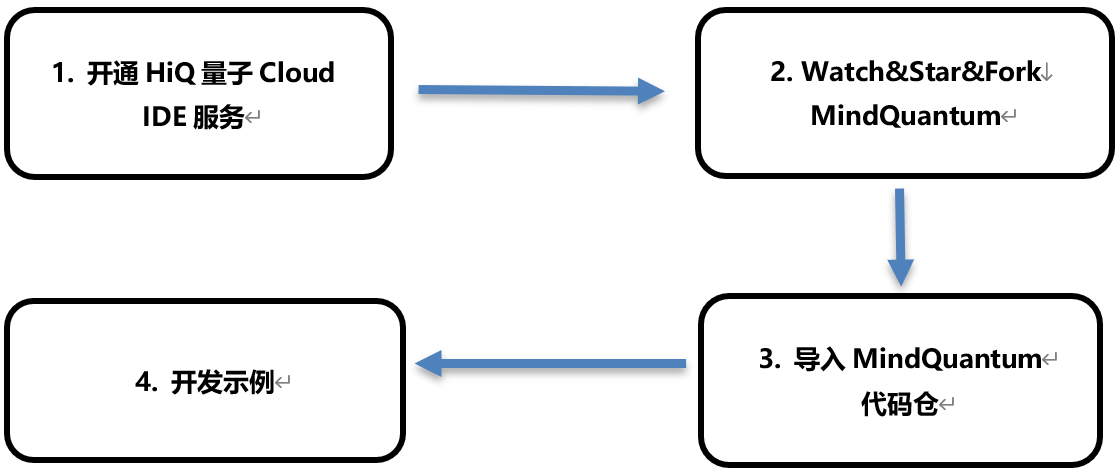
\includegraphics[width=0.5\linewidth]{1.png} % 插入svg出了点问题
%     \caption{1.svg}
%     \label{fig:enter-label}
% \end{figure}

% \end{document}


\subsection{Quantum Circuit}
实现:就是量子门集合

添加量子门的方法:
1. +=
2. circuit.x
3. list

展示线路的方法:svg

介绍常用接口:
1. n_qubits(包含多少比特)
2. params_name(有哪些变量)
3. has_measure_gate(是否含有测量)
4. matrix()(获取线路矩阵)
5. get_qs()(获取量子态)
6. summary()

高阶操作:
1. 线路压缩
2. 更改比特顺序
3. 更改变量名

\subsection{Quantum Operator}
% \begin{lstlisting}
% 理论与实现:
% 1. 费米子
% 2. 玻色子
% 3. mq中如何构造这些算子

% 支持功能:
% 1. 运算
%   a. 算子间相乘
%   b. 加上一个数
% 2. Transfrom
% \end{lstlisting}
View demo code of this section: \democode{02}{2.4}

Simulating many-body physical systems was the initial application scenario proposed by Richard Feynman for quantum computers. Effective simulations of such systems can aid us in understanding and designing new materials. Among the various many-body physics models, we are particularly interested in the Heisenberg model and the Fermi-Hubbard model. The Hamiltonians for these models can be expressed as follows:

\begin{align*}
    H_\text{Heisenberg}    & = -J\sum_{<i,j>}\sigma_i\otimes \sigma_j-h\sum_i\sigma_i                                             \\
    H_\text{Fermi-Hubbard} & = -\sum_{<i,j>,\sigma}\left(a_{i\sigma}^\dagger a_{j\sigma} + a_{j\sigma}^\dagger a_{i\sigma}\right) \\
                           & + U\sum_i n_{i\uparrow}n_{i\downarrow}
\end{align*}

In \MindQuantum, it is straightforward for us to construct those hamiltonian with the help of \QubitOperator and \FermionOperator.

\subsubsection{Qubit Operators}

In Heisenberg model, $\sigma_i$ represent the pauli operator. The matrix form of pauli operator is:

\begin{align*}
    \sigma_X & = \begin{pmatrix}
                     0 & 1 \\
                     1 & 0
                 \end{pmatrix}, \sigma_Y = \begin{pmatrix}
                                               0 & -i \\
                                               i & 0
                                           \end{pmatrix} \\
    \sigma_I & =\begin{pmatrix}
                    1 & 0 \\
                    0 & 1
                \end{pmatrix}, \sigma_Z = \begin{pmatrix}
                                              1 & 0  \\
                                              0 & -1
                                          \end{pmatrix}
\end{align*}
In \MindQuantum, \QubitOperator is used to build this kind of operator. Given a pauli operator $\sigma_{X,3}\otimes \sigma_{Y,1}\otimes \sigma_{Z,0}=X_3 Y_1 Z_0$, which means apply pauli $Z$, pauli $Y$ and pauli $X$ on qubit 3, 1 and 0,  we can easily construct it with:

\begin{lstlisting}
from mindquantum.core.operators import QubitOperator

ops = QubitOperator('Z0 Y1 X3')
\end{lstlisting}
Please note that since $[Z_0, Y_1]= [Z_0,X_3] = [Y_1, X_3]=0$, so the order of pauli word in the pauli string does not matters.

\QubitOperator also support arithmetic operation, which can help you to build more complex operators:

\begin{lstlisting}
from mindquantum.core.operators import QubitOperator
from mindquantum.core.parameterresolver import ParameterResolver as PR

op1 = QubitOperator('X0')
op2 = QubitOperator('Z1', 'a')
op3 = QubitOperator('Y1')
op4 = 2 * op1 * op2 + op3 * PR('b')
print(op4)
print(op4.subs({'a':1, 'b':2}).matrix().toarray())
\end{lstlisting}
The output is:
\begin{lstlisting}
2*a [X0 Z1] +
  b [Y1]

[[ 0.+0.j  2.+0.j  0.-2.j  0.+0.j]
 [ 2.+0.j  0.+0.j  0.+0.j  0.-2.j]
 [ 0.+2.j  0.+0.j  0.+0.j -2.+0.j]
 [ 0.+0.j  0.+2.j -2.+0.j  0.+0.j]]
\end{lstlisting}
In the last line, we use \code{.subs} to set the value of parameters and get the csr format sparse matrix with \code{.matrix}.

\subsubsection{Fermion Operators}

In Fermi-Hubbard model, $a_i^\dagger$ and $a_i$ are creation and annihilation operators of fermion. Different from pauli operator, the fermion operator follows anti-commutation relation:
\begin{align*}
    \{a_i, a_j^\dagger\} & = a_ia_j^\dagger + a_j^\dagger a_i = \delta_{ij} \\
    \{a_i, a_j\}         & = \{a_i^\dagger, a_j^\dagger\}=0
\end{align*}
In qubit system, the creation and annihilation operators acting on state $\ket{0}$ and $\ket{1}$ follows:
\begin{align*}
    a\ket{0}          & =0,        & a\ket{1}          & =\ket{0} \\
    a^\dagger \ket{0} & = \ket{1}, & a^\dagger \ket{1} & =0
\end{align*}

The matrix form of creation and annihilation would be:

\begin{align*}
    a=\begin{pmatrix}
          0 & 1 \\
          0 & 0
      \end{pmatrix},
    a^\dagger=\begin{pmatrix}
                  0 & 0 \\
                  1 & 0
              \end{pmatrix}
\end{align*}
In \MindQuantum, we use \FermionOperator to construct fermion operator. Suppose we first create a state on qubit 1 and annihilate a state on qubit 0, the operator will be $a_1^\dagger\otimes a_0$, and you can build it with:
\begin{lstlisting}
from mindquantum.core.operators import FermionOperator
op1 = FermionOperator('1^ 0')
\end{lstlisting}
In the fermion string, we use \verb|^| to represent $\dagger$ and the number to tell us on which qubit that we act. The arithmetic operation of \FermionOperator is very similar with \QubitOperator, and we will not discuss it more.


\subsubsection{Operator Functions}

Mindquantum also supplies a number of advanced functions for Operators. Here are some show case:
\begin{itemize}
    \item \methodcommutator{op1}{op2} : Calculate the commutator of two operators.
          \begin{lstlisting}
from mindquantum.core.operators import QubitOperator, FermionOperator, commutator
qub_op1 = QubitOperator("X1 Y2")
qub_op2 = QubitOperator("X1 Z2")
commutator(qub_op1, qub_op1)  # 0
commutator(qub_op1, qub_op2)  # (2j) [X2]
    \end{lstlisting}
    \item \methodcountqubits{op1} : Count the number of qubits before deleting unused qubits.
          \begin{lstlisting}
from mindquantum.core.operators import QubitOperator,FermionOperator, count_qubits
qubit_op = QubitOperator("X1 Y2")
count_qubits(qubit_op)  # 3
fer_op = FermionOperator("1^")
count_qubits(fer_op)  # 2
    \end{lstlisting}
    \item \methodhermitianconj{op1} : Get the hermitian conjugation of given operator.
          \begin{lstlisting}
from mindquantum.core.operators import FermionOperator, hermitian_conjugated
fer_op = FermionOperator("1^ 3")
hermitian_conjugated(fer_op)
    \end{lstlisting}
\end{itemize}


\subsection{Basic Usage of Simulator}
可用的模拟器:
1. 态矢量(强调 little endian)
2. 密度矩阵
3. 张量网络

使用方法:
1. apply_gate
2. apply_circuit
3. apply_hamiltonian(介绍mq中的Hamiltonian)
4. get_expectation
5. get_expectation_with_grad
6. sampling


% \section{Features of MindSpore Quantum}

% \subsection{Gradient of Variational Quantum Algorithm}
% \begin{lstlisting}
介绍变分量子算法

介绍梯度计算方法 Adjoint Differentiation

如何优化线路:
1. scipy
2. mindspore

mq中如何实现:
1. 如何用模拟器求解线路梯度(相应接口)
2. 结合pr:
  a. 控制哪些参数需要求梯度
  b. 参数共享
  c. 支持哪些形式:1)左矢,2)右矢,3)内积

介绍mq中的贫瘠高原接口
\end{lstlisting}

% \subsection{Circuit Ansatz Library}
% 列举:以表格的形式呈现

介绍ansatz设计方法

% \subsection{Quantum Algorithm Subroutine}
% 列举:以表格的形式呈现


% \section{Circuit Simulation Backend}

% \subsection{State Vector and Density Matrix Simulator}
% \begin{lstlisting}
底层实现原理

不同硬件上的针对性加速:
1. avx
2. arm
3. 鲲鹏
4. GPU
\end{lstlisting}

% \subsection{Tensor Network Simulator}
% \begin{lstlisting}
基本原理

特有特性:
1. 单振福
2. 多振幅
3. 部分振幅

优缺点:优点:内存少、稀疏线路模拟快,大线路采样

适用场景和应用前景
\end{lstlisting}

% \subsection{Channel Based Noise Simulator}
% 噪声模拟基本理论:Kraus算符

mq中的量子信道

如何组成噪声模拟器:ChannelAdder


% \section{Applications}
% \subsection{Quantum Neural Network (Xu Zhou$^{1,2}$)}

% [1] School of Physics and Astronomy, Sun Yat-sen University, Zhuhai 519082, China\\

% [2] QUDOOR Co, Ltd., Beijing 100089, China\\

% Email: \url{zhouxu@qudoor.cn}



% 分工:苏兆峰老师课题组

鸢尾花识别:体现与mindspore结合搭建量子经典混合架构


% \subsection{Quantum Approximate Optimization Algorithm}
% 

%To run this example in the browser through Mindquantum, follow the link:

%\href{https://blog.csdn.net/fisherish/article/details/105115272}{https://blog.csdn.net/fisherish/article/details/105115272}
%\cite{PhysRevLett.131.030402} 
\subsubsection{Background}

In this section, we present an introduction to the Quantum Approximate Optimization Algorithm (QAOA) and demonstrate its implementation using Mindquantum. Additionally, we explore advanced applications in Section D, where we apply techniques STA to achieve improved convergence ansatz CD-QAOA\cite{PhysRevResearch.4.013141}.


QAOA is a powerful quantum algorithm designed to address combinatorial optimization problems by harnessing the capabilities of quantum computers. It was first proposed by Farhi et al. in 2014\cite{farhi2014quantum}, and since then, numerous variants have been developed to overcome the limitations of the original algorithm.

Inspired by the trotterized version of the quantum adiabatic algorithm, QAOA is categorized as a variational quantum algorithm. The conventional QAOA comprises two main components: the quantum part, which involves a parameterized circuit ansatz, and the classical part, responsible for optimizing these parameters. To employ the QAOA algorithm effectively, we define the problem as finding the ground state of a problem Hamiltonian. The ansatz is constructed from two fundamental building blocks, namely the mixer layer and the problem layer:

\begin{equation}
    U(\gamma, \beta) = \prod_{l=1}^p e^{-i\beta_l \hat{H}_{m}}e^{-i\gamma_l\hat{H}{{p}}}
\end{equation}
where $\hat{H}_{{m}} = \sum_i \hat{\sigma}^x_i$ represents the mixer Hamiltonian, where $\hat{\sigma}^x$ corresponds to the Pauli $x$ operator. On the other hand, $\hat{H}_{{p}}$ denotes the problem Hamiltonian.

The quantum state begins from the ground state of $\hat{H}_{\text{mixer}}$, which is $|\psi_0\rangle=|+\rangle^{\otimes n}$. Then, the quantum state for the QAOA ansatz is expressed as:
\begin{equation}
    |\psi_p(\gamma, \beta)\rangle = e^{-i\beta_p\hat{H}_m}e^{-i\gamma_p\hat{H}_p}\cdots e^{-i\beta_1\hat{H}_{m}}e^{-i\gamma_1\hat{H}_{p}}|\psi_0\rangle
\end{equation}
To determine the cost or objective function, we calculate the expectation value of the problem Hamiltonian $\hat{H}_{\text{prob}}$ with respect to the ansatz state $|\psi_p(\gamma, \beta)\rangle$. This involves performing repeated measurements of the final state in the computational basis:
\begin{equation}
    F_p(\gamma, \beta) =\langle\psi_p(\gamma, \beta)|\hat{H}_{p} |\psi_p(\gamma,\beta)\rangle
\end{equation}
The primary objective of the QAOA is to find the optimal parameters $(\gamma^*, \beta^*)$ that minimize the expectation value $F_p(\gamma, \beta)$. Achieving this goal involves employing a classical optimization algorithm to iteratively update the parameters $\gamma$ and $\beta$:
\begin{equation}
    (\gamma^*, \beta^*) = \text{arg}\min_{\gamma, \beta} F_p(\gamma, \beta)
\end{equation}

By finding these optimal parameters, QAOA enables quantum computers to efficiently tackle complex optimization challenges, offering a promising avenue for various practical applications.




\subsubsection{Implement}

For this tutorial, we use QAOA algorithm to handle the Max-Cut problem,  which is an NP-complete problem in graph theory. As shown in figure \ref{5.1_QAOA}, it needs to divide the vertices of a graph into two parts and make the most edges be cut. But when the number of vertices in the graph increases, it is difficult for us to find an effective classical algorithm to solve the Max-Cut problem, because it is very likely that there is no polynomial time algorithm for this type of NP-complete problem.

\begin{figure}[H]
    \centering
    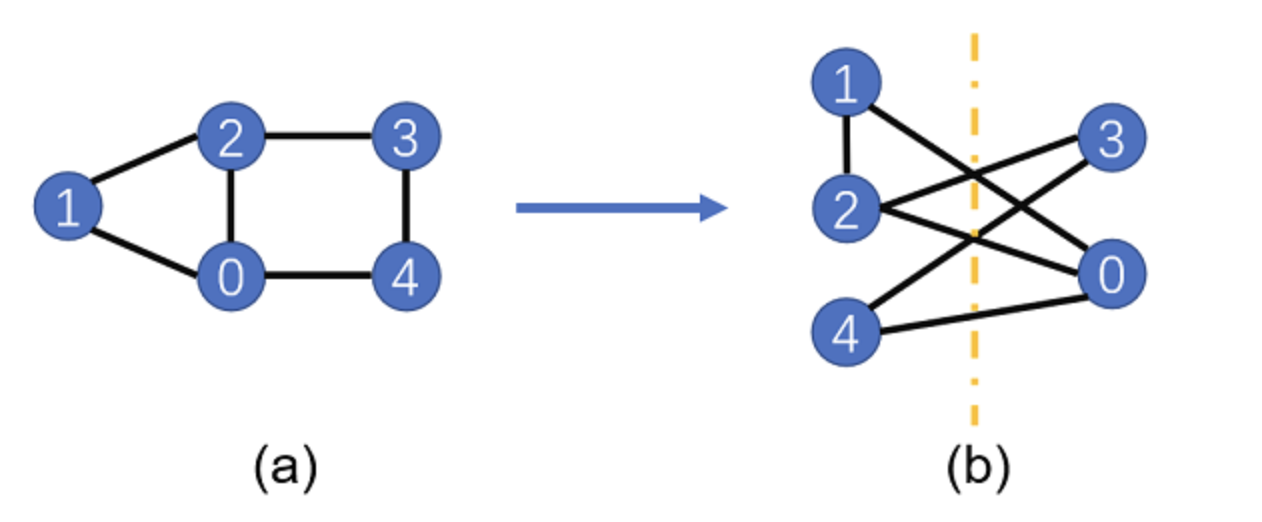
\includegraphics[width=0.49\textwidth]{5.2_figures/5.2_QAOA}
    \caption{Max-cut graph}
    \label{5.1_QAOA}
\end{figure}

Let us first generate a graph structure consisting of five vertices and six edges using NetworkX[cite].
\begin{lstlisting}
g = nx.Graph()
nx.add_path(g, [0,1])
nx.add_path(g, [1,2])
nx.add_path(g, [2,3])
nx.add_path(g, [3,4])
nx.add_path(g, [0,4])
nx.add_path(g, [0,2])
nx.draw(g,with_labels=True, font_weight='bold')
\end{lstlisting}

For QAOA algorithm, first we need to convert the Max-Cut problem into a Hamiltonian, it's ground state energy is solution of the problem. The problem hamitonian of the Max-Cut problem can be built as
\begin{equation}
    \hat{H} = \sum_{i,j\in C}(\hat{Z}_i\hat{Z}_j-1)/2
\end{equation}
where $C$ is the set of all edges. In the following function, ${ build \_ ham}$, the corresponding Hamiltonian can be constructed by inputting the graph.
\begin{lstlisting}
def build_ham(g):
    hc = QubitOperator()
    for i in g.edges:
        hc += QubitOperator(f'Z{i[0]} Z{i[1]}')
    return hc
\end{lstlisting}
Next, construct the QAOA ansatz, in which function $build\_hc$ and $build\_hb$ construct the quantum circuit according to the problem Hamiltonian and the mixer Hamiltonian. The ansatz can be directly builded in function $build\_ansatz$ by inputting the graph.

\begin{lstlisting}
def build_hc(g,para):
    hc = Circuit()
    for i in g.edges:
        hc += ZZ(para).on(i)
    return hc
def build_hb(g, para):
    hc = Circuit()
    for i in g.nodes:
        hc += RX(para).on(i)
    return hc
def build_ansatz(g, p):
    c = Circuit()
    for i in range(p):
        c += build_hc(g,f'g{i}')
        c += build_hb(g,f'b{i}')
    return c
\end{lstlisting}

In this example, p = 4 is selected, indicating that the four-layer QAOA quantum circuit is used.  And ${\rm init\_state\_circ}$ is a quantum circuit for preparing a initial state on a uniformly superposed state.
\begin{lstlisting}
p = 4
ham = Hamiltonian(build_ham(g))
ansatz = build_ansatz(g, p)
init_state_circ = UN(H, g.nodes)
\end{lstlisting}

The goal of QAOA is to find the optimal parameters that make the cost function or the expectation of hamitonian $\mathcal{E}=\langle \psi(\gamma^*, \beta^*)|\hat{H}|\psi(\gamma, \beta)\rangle$ minimize.
This problem does not require a coding-layer quantum circuit, so we use MQAnsatzOnlyLayer as a quantum neural network to be trained and the adam as the optimizer.
\begin{lstlisting}
import mindspore as ms
ms.set_context(mode=ms.PYNATIVE_MODE, device_target="CPU")

total_circuit = init_state_circ + ansatz
sim = Simulator('mqvector', total_circuit.n_qubits)
grad_ops = sim.get_expectation_with_grad(ham, total_circuit)
net = MQAnsatzOnlyLayer(grad_ops)
opti = nn.Adam(net.trainable_params(), learning_rate=0.05)
train_net = nn.TrainOneStepCell(net, opti)

for i in range(600):
    if i%10 == 0:
        print("train step:", i, ", cut:", (len(g.edges)-train_net())/2)
\end{lstlisting}
\begin{lstlisting}
train step: 0 ,   cut: [3.0001478]
train step: 10 ,  cut: [4.1718774]
train step: 20 ,  cut: [4.6871986]
train step: 30 ,  cut: [4.7258005]
train step: 40 ,  cut: [4.804503]
train step: 50 ,  cut: [4.8477592]
train step: 60 ,  cut: [4.8705964]
train step: 70 ,  cut: [4.9060946]
train step: 80 ,  cut: [4.933446]
train step: 90 ,  cut: [4.9356637]
train step: 100 , cut: [4.938308]
train step: 110 , cut: [4.9390197]
train step: 120 , cut: [4.939068]
train step: 130 , cut: [4.9392157]
train step: 140 , cut: [4.939249]
train step: 150 , cut: [4.939247]
train step: 160 , cut: [4.939255]
train step: 170 , cut: [4.939257]
train step: 180 , cut: [4.939257]
train step: 190 , cut: [4.939257]
\end{lstlisting}

According to the above training results, we found that the number of edge cuts corresponding to the ground state energy of the Hamiltonian of this problem approaches 5.

In mindquantum,  we can directly import the function $MaxCutAnsatz$ to build ansatz for the maxcut problem.
\begin{lstlisting}
import numpy as np
from mindquantum.algorithm.nisq import MaxCutAnsatz
graph = [(0, 1), (1, 2), (0, 2)]
p = 1 # layer
maxcut = MaxCutAnsatz(graph, p)
maxcut.circuit.svg()
\end{lstlisting}
\begin{figure}[H]
    \centering
    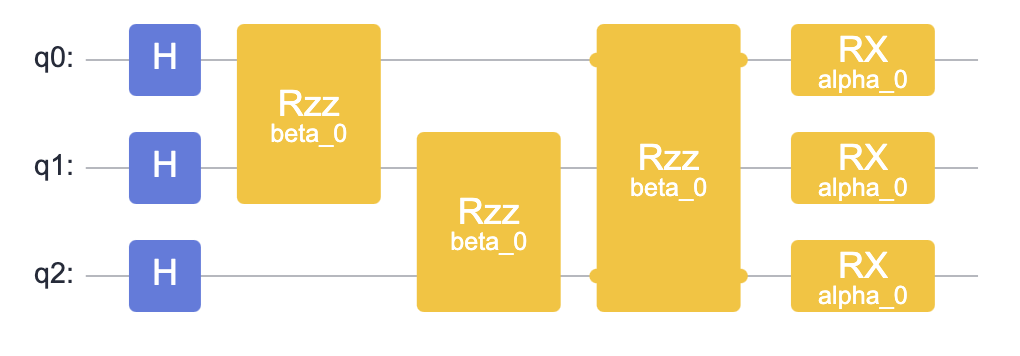
\includegraphics[width=0.49\textwidth]{5.2_figures/5.2_QAOA_ansatze}
    \caption{Max-cut problem Ansatze}
    \label{5.1_QAOA}
\end{figure}
At the same time, the Hamiltonian can also be obtained
\begin{lstlisting}
print(maxcut.hamiltonian)
\end{lstlisting}
\begin{lstlisting}
3/2 [] +
-1/2 [Z0 Z1] +
-1/2 [Z1 Z2] +
-1/2 [Z0 Z2]
\end{lstlisting}
The cutting scheme of the MaxCut problem and the number of cutting edges of the cutting scheme can be obtained through the function $get\_partition$ and $get\_cut\_value$. The cutting scheme is a list array consisting of two list arrays, and each list array contains the cut nodes.
\begin{lstlisting}
partitions = maxcut.get_partition(5, np.array([4, 1]))
for i in partitions:
    print(f'partition: left: {i[0]}, right: {i[1]}, cut value: {maxcut.get_cut_value(i)}')
\end{lstlisting}
\begin{lstlisting}
partition: left: [0, 2],   right: [1], cut value: 2
partition: left: [1, 2],   right: [0], cut value: 2
partition: left: [1],   right: [0, 2], cut value: 2
partition: left: [0, 1, 2], right: [], cut value: 0
partition: left: [], right: [0, 1, 2], cut value: 0
\end{lstlisting}












% \subsection{Variational Quantum Eigensolver}
% 分工:ab老师课题组

% % \subsection{Advanced Quantum Aplications}
% % \subsection{CD QAOA}


%To run this example, follow the link

\subsubsection{Background}
In the field of quantum computing, researchers are continuously seeking efficient and robust methods to tackle complex problems. Adiabatic quantum computation (AQC) is one such approach, where a quantum system evolves gradually from an initial Hamiltonian to a final Hamiltonian that encodes the desired solution. According to the adiabatic theorem, if this evolution is slow enough, the system will remain in the ground state of the Hamiltonian throughout the process:

\begin{equation}
H(t) = (1-\lambda(t))H_{\text{initial}} + \lambda(t)H_{\text{final}},
\end{equation}

where $\lambda(t)\in[0,1]$. However, implementing AQC in practical scenarios faces challenges arising from external noise, imperfections, and the need for long evolution times. To overcome these limitations and enhance the efficiency of adiabatic evolution, one promising approach to solve this problem is the Quantum Approximate Optimization Algorithm (QAOA), where a parameterized quantum circuit (ansatz) prepares a trial state to approximate solutions for optimization problems. By optimizing the ansatz parameters, QAOA seeks to find the optimal values that minimize or maximize the objective function, which encodes the problem's energy landscape.

However, practical implementations of QAOA face challenges due to noise, decoherence, and the complexity of parameter optimization. To enhance its performance and robustness, the Counterdiabatic Quantum Approximate Optimization Algorithm (CD-QAOA) introduced the counterdiabatic (CD) term:
\begin{equation}
H_{\text{CD-QAOA}} = (1 - \lambda(t))H_{\text{initial}} + \lambda(t)H_{\text{final}} + H_{\text{CD}},
\end{equation}
It combines ideas from both AQC and the Quantum Approximate Optimization Algorithm (QAOA) by introducing one additional parameter per layer compared to QAOA. This results in shallower quantum circuits without compromising accuracy:
\begin{equation}
U(\gamma, \beta)\to U(\gamma, \beta, \alpha), \quad F(\gamma, \beta)\to F(\gamma, \beta, \alpha),
\end{equation}
where $\alpha, \beta, \gamma$ represents the digitized parameters, $F$ is cost function and $U$ is evolution operator..
The CD term acts as an extra component in the Hamiltonian and is carefully designed based on the instantaneous eigenstates and eigenenergies of the evolving Hamiltonian.  The counterdiabatic term effectively suppresses errors and reduces the required evolution time, leading to enhanced efficiency and reliability in quantum computations.

To derive the precise form of the counterdiabatic term, various techniques, such as Lewis-Riesenfeld invariants and transitionless quantum driving, have been applied. The implementation of the CD term is tailored to the specific problem and dynamics of the quantum system, utilizing available control techniques. In cases where obtaining exact CD terms becomes challenging, an approximate CD driving approach is proposed, utilizing the nested commutator method\cite{Chandarana_2023} with the adiabatic gauge potential:

\begin{equation}
A_{\lambda}^{(l)} = i\sum_{k=1}^{l}\alpha_{k}(t)[H_{a},[H_{a},...[H_{a}, \partial_{\lambda}H_{a}]]].
\end{equation}

DC-QAOA holds promise for solving a wide range of optimization problems, from combinatorial optimization to machine learning tasks and financial portfolio optimization. As quantum computing technology continues to advance, DC-QAOA represents an exciting avenue for leveraging the counterdiabatic term and parameter space digitization to unlock new frontiers in quantum optimization.

\textbf{Target problem}
\begin{itemize}
\item[1.] Learn how to find the ground state of problem Hamiltonian
\item[2.] Utilize quantum circuits to find optimized parameters 
\end{itemize}
\textbf{Required Mindquantum functionalities}
\begin{itemize}
\item[1.] gradient-based optimizer
\item[2.] Batch quantum circuit simulator

\end{itemize}

\subsubsection{Implement}
As a mature application of QAOA, this algorithm requires two steps, which is building the ansatz circuit and optimization. Now let's look at how to implement Digitized-counterdiabatic quantum approximate optimization algorithm (DC-QAOA) into Ising spin model, the model is depicted in Fig.~\ref{fig:ising}. The initial state is choose as $H_{initial} = \sum_{i}\sigma_{i}^{x}$. The general form of the Hamiltonian of the 1D Ising spin model is given by
\begin{figure}
    \centering
    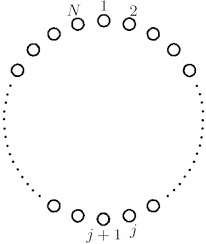
\includegraphics[width=0.5\linewidth]{5.4.1_figure/ising.jpg}
    \caption{Schematic picture of the Ising model}
    \label{fig:ising}
\end{figure}

\begin{equation}
H_{final} = -\sum_{\langle i,j \rangle}J_{ij}\sigma_{i}^{z}\sigma_{j}^{z} - \sum_{i}h_{i}\sigma_{i}^{z} - \sum_{i}k_{i}\sigma_{i}^{x}.
\end{equation}
\begin{lstlisting}
# generate H_{initial} as H_{mixer}
# n_qubits is the number of qubits
def generate_h_mixer(n_qubits:int):
    h_mixer = QubitOperator()
    for i in range(n_qubits):
        h_mixer += QubitOperator(f'X{i}')
    return h_mixer
    
# generate H_{final} as H_{prob}
def generate_h_prob(n_qubits:int, J:float, h:float, k:float):
    h_prob = QubitOperator()
    for i in range(n_qubits):
        j = (i+1)%n_qubits
        h_prob += QubitOperator(f'Z{i} Z{j}', J)
        h_prob -= QubitOperator(f'Z{i}', h)
        h_prob -= QubitOperator(f'X{i}', k)
    return h_prob
\end{lstlisting}

In our case,  a pool of CD operators is defined using the nested commutator approach of the adiabatic gauge potential \cite{PhysRevResearch.4.013141}
$$A = \{\sigma^{y},\sigma^{z}\sigma^{y}, \sigma^{y}\sigma^{z}, \sigma^{x}\sigma^{y}, \sigma^{y}\sigma^{x} \}.$$

Here we present a 12 qubits system and we consider second-order $A = \sum_{i}\sigma_{i}^{z}\sigma_{i+1}^{y}$. For simplify, we choice  $J = -1, h = 0, k = -1$. Following we build an ansatz layer for DC-QAOA.
\begin{lstlisting}
def generate_h_cd(n_qubits:int):
    h_cd = QubitOperator()
    for i in range(n_qubits-1):
        h_cd += QubitOperator(f'Z{i} Y{i+1}')
    return h_cd
\end{lstlisting}    

\begin{lstlisting}
n_qubits = 12
J, h, k = -1, 0, -1

h_prob = generate_h_prob(n_qubits, J, h, k)
h_mixer = generate_h_mixer(n_qubits)
h_cd = generate_h_cd(n_qubits)
\end{lstlisting}

In order to prepare the eigenstate for $H_{initial}$, we first put ${\rm prep\_circ}$, and then apply evolution operator on it. 
\begin{lstlisting}
# generate the eigenstate for $H_{mixer}$
prep_circ = UN(H, n_qubits)

# choose two layer 
p = 3
ansatz_template = u_p + u_m + u_cd

ansatz = Circuit() + prep_circ
for i in range(p):
    ansatz += add_suffix(ansatz_template, str(i)) + BarrierGate()
\end{lstlisting}

As long as we have set up the ansatz circuit, we can change the number of layers or type of optimizer in order to find the optimal parameter set. We define cost function using 
\begin{equation}
E = \left<\psi_0\right|U^{\dagger}\ H_{prob} U\left|\psi_0\right>,
\end{equation}
where $U = \Pi_{i=0}^3 U_{cd}(\alpha_i)U_m(\beta_i)U_p(\gamma_i)$ and this is just the evolution operator. 
\begin{lstlisting}
energys = []
# define cost function
def fun(x0, grad_ops, energys):
    f, g = grad_ops(np.array(x0))
    f = np.real(f[0, 0])
    g = np.real(g[0, 0])
    energys.append(f)
    if len(energys)%5==0:
        print(f"step: {len(energys)}, energy: {f}")
    return f, g
\end{lstlisting}

In this tutorial, we will optimize the gradient using BFGS optimizer\cite{chandarana2022meta}, which will have good enough results. If you plot the figure of mean energy, you will have result like Fig.~\ref{fig:dc}. Here, the green line is the exact eigenvalue of $H_{prob}$, the blue line is the mean value during the optimizing process, the orange line is QAOA with three layers. We can notice that DC-QAOA  has converged to the exact value in 70 steps within 0.5s. Comparing these two algorithm from the ability of estimating the ground state, DC has advantage over QAOA.
\begin{figure}
    \centering
    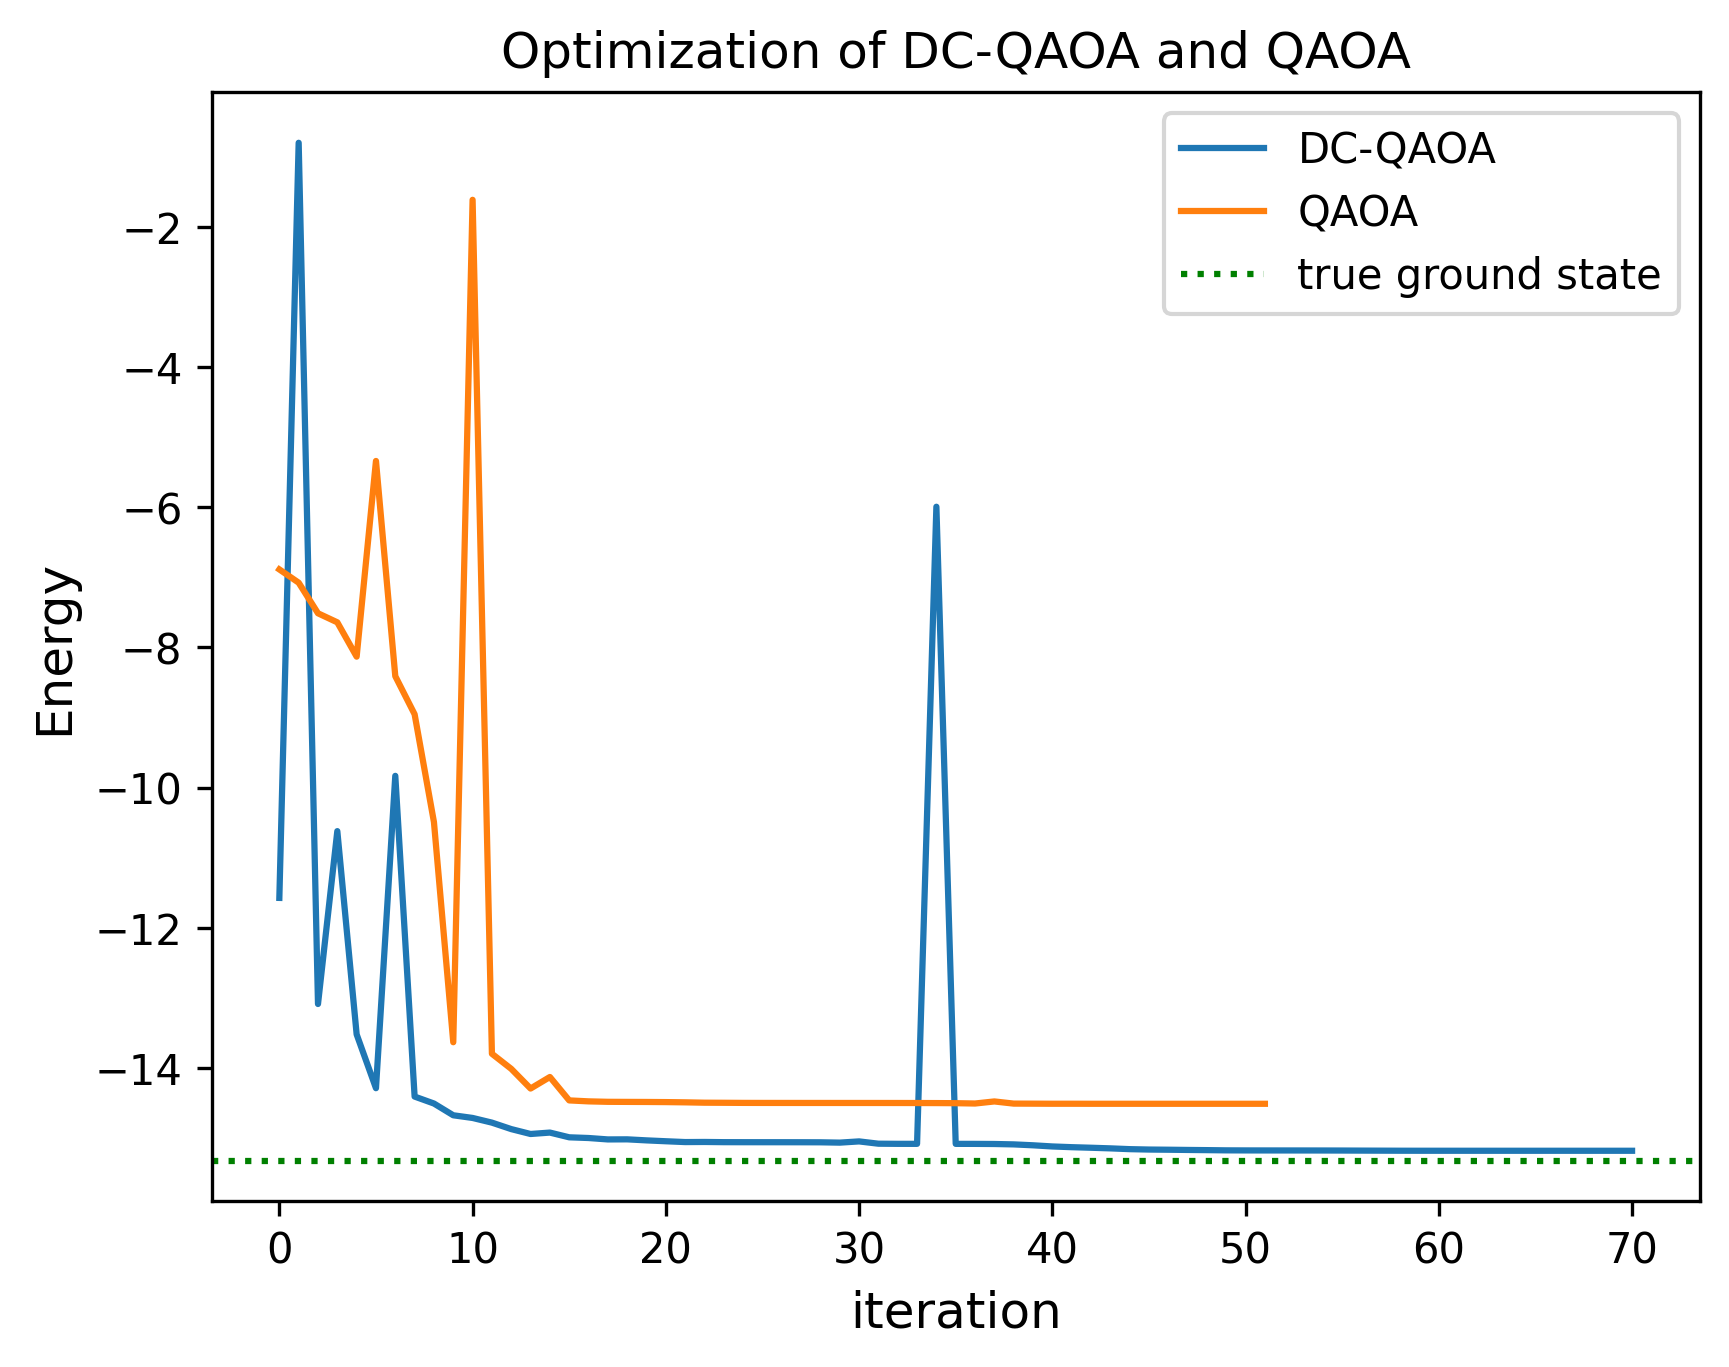
\includegraphics[width = 1 \linewidth]{5.4.1_figure/DC-WHITE.png}
    \caption{Mean Energy vs. iteration time}
    \label{fig:dc}
\end{figure}





\subsection{Symmetry enhanced VQE}
The study of variational quantum algorithms has largely been focused on identifying the ground state of intricate many-body systems. In this context, the Variational Quantum Eigensolver (VQE) algorithm has emerged as a potent tool, designed to target the ground state of a many-body system by minimizing average energy. However, several critical phenomena in physics, including topological phases, necessitate knowledge of several low-energy eigenstates, not just the ground state. Therefore, the generalization of VQE to higher energy eigenstates is highly important.

The weighted SSVQE provides an alternative method to generate all the $k$ lowest energy eigenstates of a given Hamiltonian $H$~\cite{?}. This method utilizes a set of $k$ orthogonal initial states, denoted as $\{|\phi_{i}\rangle\}_{i=1}^{k}$ (where $\langle \phi_{i} | \phi_{j} \rangle = \delta_{ij}$), as the input of a single parameterized quantum circuit, described by the unitary operator $U(\vec{\theta})$. Given that the initial states are orthogonal, the outputs $U(\vec{\theta})| \phi_{j} \rangle$, generated by the same circuit, maintain orthogonality. In the weighted SSVQE, the objective is to minimize the cost function
\begin{equation}
    \mathrm{cost} = \sum_{i=1}^{k} w_{i} \langle \phi_{i}| U^{\dagger}(\vec{\theta}) H U(\vec{\theta}) | \phi_{i} \rangle
    \label{ssvqe_cost}
\end{equation}
where $w_1 > w_2 > \cdots > w_k$ are real positive numbers. Minimizing the cost function in Eq.~\eqref{ssvqe_cost} produces all the $k$ lowest energy eigenstates such that $|E_{i}\rangle = U(\vec{\theta}^{*})|\phi_{i}\rangle$.
A notable advantage of the weighted SSVQE is that it delivers all the $k$ lowest energy eigenstates through a single optimization process, without requiring any overlap of quantum states. However, the algorithm becomes more resource-demanding as the number of target eigenstates increases.

Symmetry is one of the most profound concepts in physics, especially in quantum mechanics. A majority of physical systems exhibit various types of symmetries that can be accurately described mathematically. The VQE algorithm can also significantly benefit from the integration of these symmetries. There are two ways to incorporate symmetries in the VQE algorithms: (i) designing the circuit to naturally generate the quantum states with the relevant symmetry~\cite{?}, and (ii) adding extra terms to the cost function to penalize the quantum states without the relevant symmetry~\cite{?}.


Leveraging the adaptability and comprehensive capabilities of MindQuantum, researchers are able to work with any optimization target by defining custom objective functions. Here, we present an example of implementing SSVQE through MindQuantum to accurately determine the four lowest state energies of the Heisenberg Hamiltonian, employing different symmetry incorporation strategies.


The full notebook and implementation is available at:
XXXXXXXXX

First, we need to construct the symmetry preserving ansatz~\cite{?}.
\begin{lstlisting}
def entangling_gate(parameter, qubits):
    circuit = Circuit()
    circuit += RZ(-np.pi / 2).on(qubits[1])
    circuit += CNOT.on(qubits[0], qubits[1])
    circuit += RZ({parameter: -2}).on(qubits[0])
    circuit += RZ(np.pi / 2).on(qubits[0])
    circuit += RY({parameter: 2}).on(qubits[1])
    circuit += RY(-np.pi / 2).on(qubits[1])
    circuit += CNOT.on(qubits[1], qubits[0])
    circuit += RY({parameter: -2}).on(qubits[1])
    circuit += RY(np.pi / 2).on(qubits[1])
    circuit += CNOT.on(qubits[0], qubits[1])
    circuit += RZ(np.pi / 2).on(qubits[0])
    return circuit

def ansatz(N, layers, local_rot=True):
    circuit = Circuit()
    params_index = 0
    for layer_index in range(layers):
        for i in range(2):
            for j in range(i, N - 1, 2):
                circuit += entangling_gate(str(params_index), [j, j + 1])
                params_index += 1
        if local_rot:
            for i in range(N):
                circuit += PhaseShift(params_index).on(i)
                params_index += 1
    return circuit
\end{lstlisting}

The SSVQE can then be implemented as a combination of several VQEs with distinct initialization circuits yet utilizing a shared parameter ansatz. One need to ensured that the resulting states post-initialization are orthogonal.
For each VQE, a unique measurement function can be defined to accomplish a variety of tasks.
Using the "get\_expectation\_with\_grad" function, one can easily obtain the expectation value and the corresponding gradient with respect to the trainable variables. Here, as an example, we demonstrate the code implementation for obtaining the second and the third lowest state energies of the Heisenberg Hamiltonian. In this particular instance,
we use a $S_z$-conserving ansatz, which preserves the $z$ component of the total spin, and the total spin operator is added to the cost function as a penalty term. The cost function is then modified into a form of
\begin{equation}
    \mathrm{cost} = \sum_{i=1}^{k} w_{i} \langle \phi_{i}| U^{\dagger}(\vec{\theta}) [H + (\hat{O} - c)^2] U(\vec{\theta}) | \phi_{i} \rangle,
    \label{ssvqe_cost_pen}
\end{equation}
where $c$ is a constant indicating the target subspace. Here, we do the expansion $(\hat{O} - c)^2 {=} \hat{O}^2 {-} c\hat{O} {+} c^2$. Together with the Hamiltonian, now we have three different measurement operators.

\begin{lstlisting}
class SSVQE:
    def __init__(self, n_qubits, init_circuits, pqc, ops):
        self.n_qubits = self.n_qubits
        self.circs = [circ + pqc for circ in init_circuits]
        self.sim = Simulator('mqvector', n_qubits)
        self.grad_ops = [self.sim.get_expectation_with_grad(ops, circ) for circ in circs]
    
    def __call__(self, inputs):
        cost = 0
        cost_grad = 0
        for i in range(len(self.grad_ops)):
            f, g = self.grad_ops[i](inputs)
            f1, f2, f3 = f[0, 0].real, f[0, 1].real, f[0, 2].real
            g1, g2, g3 = np.array(g[0, 0, :].real), np.array(g[0, 1, :].real), np.array(g[0, 2, :].real)
            cost += (f1 + f2 + f3) * (len(self.grad_ops) - i)
            cost_grad += (g1 + g2 + g3) * (len(self.grad_ops) - i)
        return cost, cost_grad
\end{lstlisting}

Now we need to set up the training function for the SSVQE. With all the module we predefined, the procedure is straightforward. The choice of the classical optimizer is flexible as well, here we choose the "L-BFGS-B" optimizer implemented in SciPy.

\begin{lstlisting}
def training(ssvqe, optimizer):
    initial_parameter = (np.random.rand(len(ssvqe.circs[0].params_name)) - .5) * np.pi
    result = optimizer.minimize(ssvqe, initial_parameter, jac=True, method='l-bfgs-b')
    return result
\end{lstlisting}

This implementation takes several minutes to finish training. One can track the results after each optimization step and generate a plot to compare the approximation results with the actual energies. In Fig.~\ref{}, we show the simulation results for the four lowest state energies of the Heisenberg Hamiltonian. It is clear to see that, incorporating SSVQE with the inherent symmetries, one can approximate both the ground and excited state energies precisely in a resource-efficient manner.

\subsection{Data-reuploading Classifier}
\input{5.4.3_Data-reuploading_Classifier}

\subsection{Q-GAN}
分工:舒润秋

\subsection{Reinforcement Learning}
\textit{Introduction} -- An overall reinforcement learning algorithm(RL) is composed of Agent, Environment, State, Action, and Reward. After the Agent executes an action, the Environment switches to a new State according to the Action and gives a Reward according to certain rules. After that, the Agent updates its decision-making process according to the obtained new State and Reward and gives a new Action, and so on, until the entire control process is completed. We denote $\pi_{\theta}$ as the policy function, $s$ as each state of the environment, $r$ as the reward in each state, and $a$ as the action of the agent. The architecture of RL is demonstrated in Figure~\ref{RL_frame}.
\begin{figure}[ht]
  \centering
  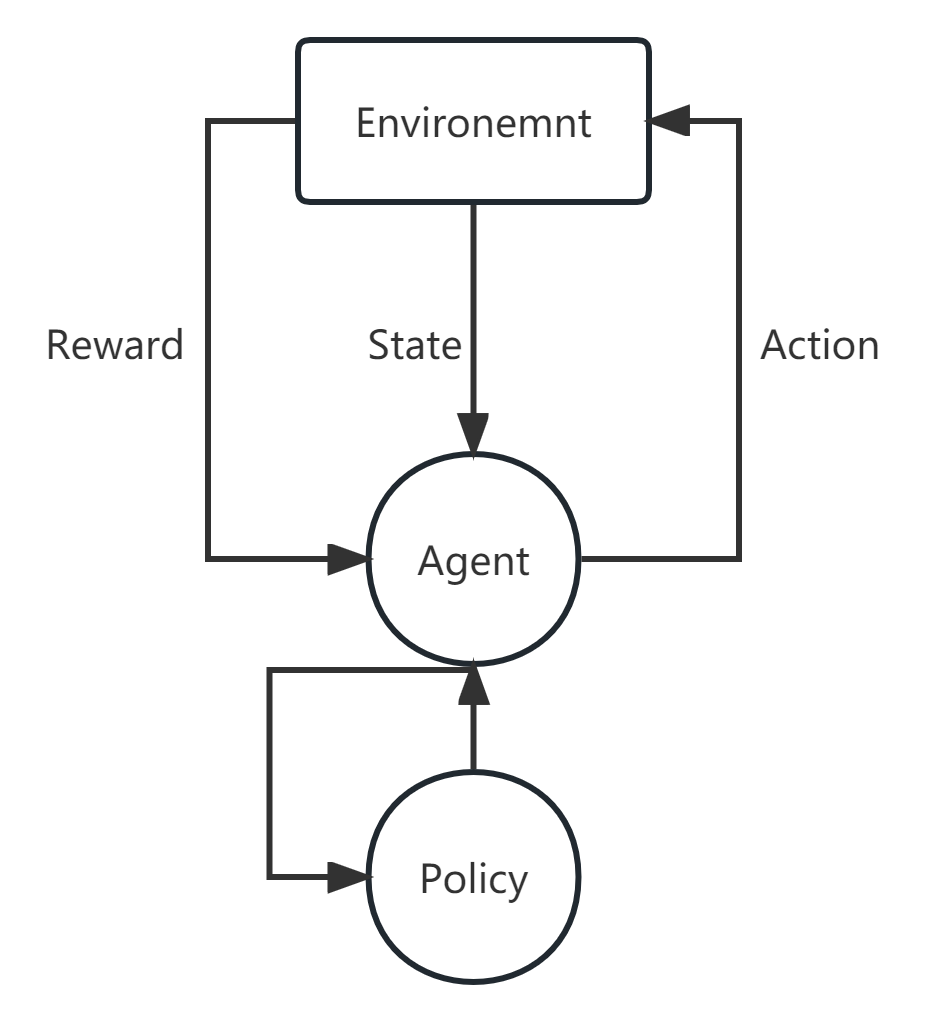
\includegraphics[scale=0.4]{tex/5.4.5_RL/RL.png}
  \caption{\label{RL_frame} The demonstration of RL wroking process.}
\end{figure} 

We assumed an environment has $N$ different states. And we act action $a_{i-1}$ on state $s_{i-1}$ with the result $s_{i}$. The transition probability function from state $s_{i-1}$ to state $s_{i}$ can be $P(s_{i+1}|s_{i},a_{i})$. Meanwhile, there is a reward $r_i$ in each state calculated by reward function $R_i=R(a_i,s_i,s_{i-1})$. In the progress of environmental change, the reward expectation is only determined by the latest $state$, which is called the Markov decision process. Therefore, each $T$ step trajectory will be chosen by the agent with probability:

\begin{equation}
    \begin{split}
        &P(\tau|\pi_{\theta})=\\
        &\rho(s_0)\prod_{k=0}^{k=T-1}P(s_{k+1}|s_{k},a_{k})\pi_{\theta}(a_{k}|s_{k})
    \end{split}
\end{equation}
where $\rho$ is the initial state distribution. Then the expectation of $T$ steps trajectory's reward is:
\begin{equation}
    \eta(\pi_{\theta})=\int_{\tau}P(\tau|\pi_{\theta})R(\tau)d\tau
\end{equation}
In order to get the optimal policy function $\pi_{\theta}$, the agent is trained to maximize the expectation $\eta$, which is:
\begin{equation}
    \pi_{\theta}^{opt}=\mathrm{argmax}_{\theta}\eta(\pi_{\theta})
\end{equation}
In following sections, we will demonstrate how to the agent in quantum devise.
\textit{Hybrid Deep Q-Network} -- Replace the neural network in the classical Deep Q-network's agent with the quantum variational circuit, we get the hybrid deep Q-network(HDQN)~\cite{Q_rl}. The architecture of HDQN is illustrated in FIG. We calculate the parameters $\theta$ by classical neural network and use them to construct the quantum variational circuit. Finally, the quantum part applies the action to the environment. Meanwhile, the environment responds with a reward $r_i$. We denote $e_i=(s_i,a_i,r_{i+1},s_{i+1})$ as a experience. In the training stage, we will use these experiences as training samples to adjust the parameters in both the classical part and quantum part according to loss function $L(\theta)$:
\begin{equation}
\begin{split}
    L(\theta_{j})=&E[R_{i+1}+\\
    &\gamma \max_{\alpha^{'}}Q(s_{i+1},a^{'},\theta_{j}^{-})-Q(s_{i},a_{i},\theta_{i})^2]
\end{split}
\label{loss func}
\end{equation}

\textit{Variational quantum circuit} -- The variational quantum circuit is a quantum circuit using adjustable parameters that can be changed by the external environment. Here, according to the architecture in ~\cite{Q_rl}, we construct the quantum circuit with the combination of encoder and ansatz. Here, we apply the Hardware Efficient circuit as the ansatz. The overall quantum circuit is illustrated in Figure~\ref{Agent_qc}.

\begin{figure*}[ht]
  \centering
  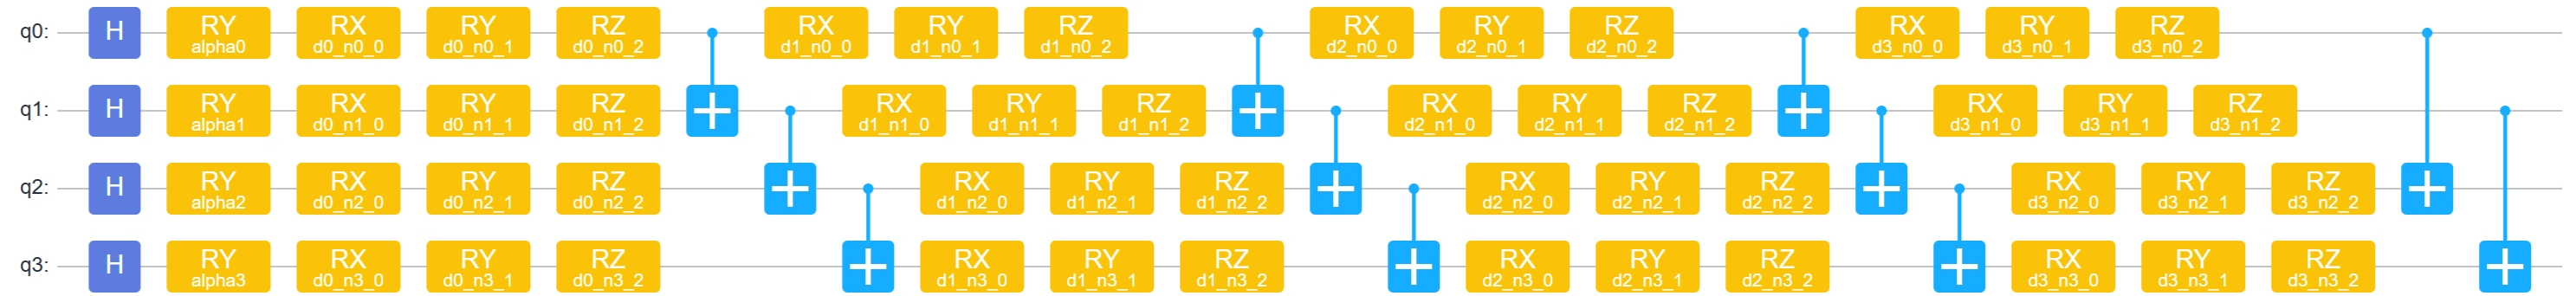
\includegraphics[scale=0.5]{tex/5.4.5_RL/Circuit.png}
  \caption{\label{Agent_qc} The overall quantum circuit of agent in RL.}
\end{figure*}

\textit{The implement in mindquantum} -- Here, we give the example of realizing HDQN by mindquantum. The first step is to construct the quantum variational circuit including the encoder and the ansatz.
\begin{lstlisting}
    def __get_encoder(self):
        encoder = Circuit()                                  
        encoder += UN(H, 4)                                  
        for i in range(4):                                   
            encoder += RY(f'alpha{i}').on(i)                  
        encoder = encoder.no_grad()                           
        quantum circuit which has no gradient: no_grad()
        encoder.summary()                                    
        return encoder
    def __get_ansatz(self):
        ansatz = HardwareEfficientAnsatz\\
            (4, single_rot_gate_seq=[RX,RY,RZ],\\
            entangle_gate=X, depth=3).circuit     
        ansatz += X.on(2,0)
        ansatz += X.on(3,1)
        ansatz.summary()                                                                              
        return ansatz
    self.circuit = self.encoder + self.ansatz
\end{lstlisting}

After the progress of the quantum circuit, we need to construct an observable Hamiltonian as a measurement basis. Here, we only measure the second and third qubits on $\sigma_y$ base. The Hamiltonian is as follows:
\begin{equation}
    H=I\otimes I\otimes\sigma_y\otimes\sigma_y
\end{equation}
We can construct the hamiltonian by mindquantum as follows:
\begin{lstlisting}
    def __get_observable(self):
        hams=[Hamiltonian(QubitOperator(f'Y{i}'))\\
            for i in [2, 3]] 
        return hams
\end{lstlisting}
Moreover, we can easily get the expectation and calculate the gradient of expectation by function $get\_expectation\_with\_grad$, which can be used to optimize parameters.

Next, we need to realize the classical part, which is a three-layers fully connected neural network with activation function Relu.
\begin{lstlisting}
    class Critic(nn.Cell):
        def __init__(self):
            super(Critic, self).__init__()
            self.relu = nn.ReLU()
            self.fc1 = nn.Dense(4, 64)
            self.fc2 = nn.Dense(64, 256)
            self.fc3 = nn.Dense(256, 1)
    
        def construct(self, x):
            x = self.relu(self.fc1(x))
            x = self.relu(self.fc2(x))
            x = self.fc3(x)
            return x
\end{lstlisting}

\textit{environment} -- Here, we focus on the problem of the gym game "CartPole-v0". It's a game that has an unbalanced cart on a track. This game has two inputs $0$ and $1$, which correspond to two directions left and right respectively. Users should control the trace moving toward these two directions and keep the cart balanced as long as possible.

The first step is to create the environment by gym.
\begin{lstlisting}
    import gym
    env = gym.make('CartPole-v0')
\end{lstlisting}
\textit{Memory buffer} -- In the progress of training, the training samples are randomly selected from the previous experience $e_i$. Therefore, we need to construct a buffer to store and sample the experience $e_i$.
\begin{lstlisting}
class Memory(object):
    ......
\end{lstlisting}
\textit{Training} -- The final step is model training. At first, we initialize HDQN with random parameters and let the actor interact with the environment. Next, we store the interaction result in the memory buffer as training samples. Finally, we sample from the memory buffer and adjust the parameters both in the classical part and quantum part with loss function (\ref{loss func}). Because of the space limitation, we will not provide the detailed code here.

\textit{Result of numerical simulation} -- In order to evaluate the result of the HDQN. We do some experiments to evaluate the performance. As shown in Figure ~\ref{stochastic} We compare the average results from multiple experiments with randomized strategy experiments. The results show that reinforcement learning using quantum circuits as the agent has indeed learned the strategy.
\begin{figure}[ht]
  \centering
  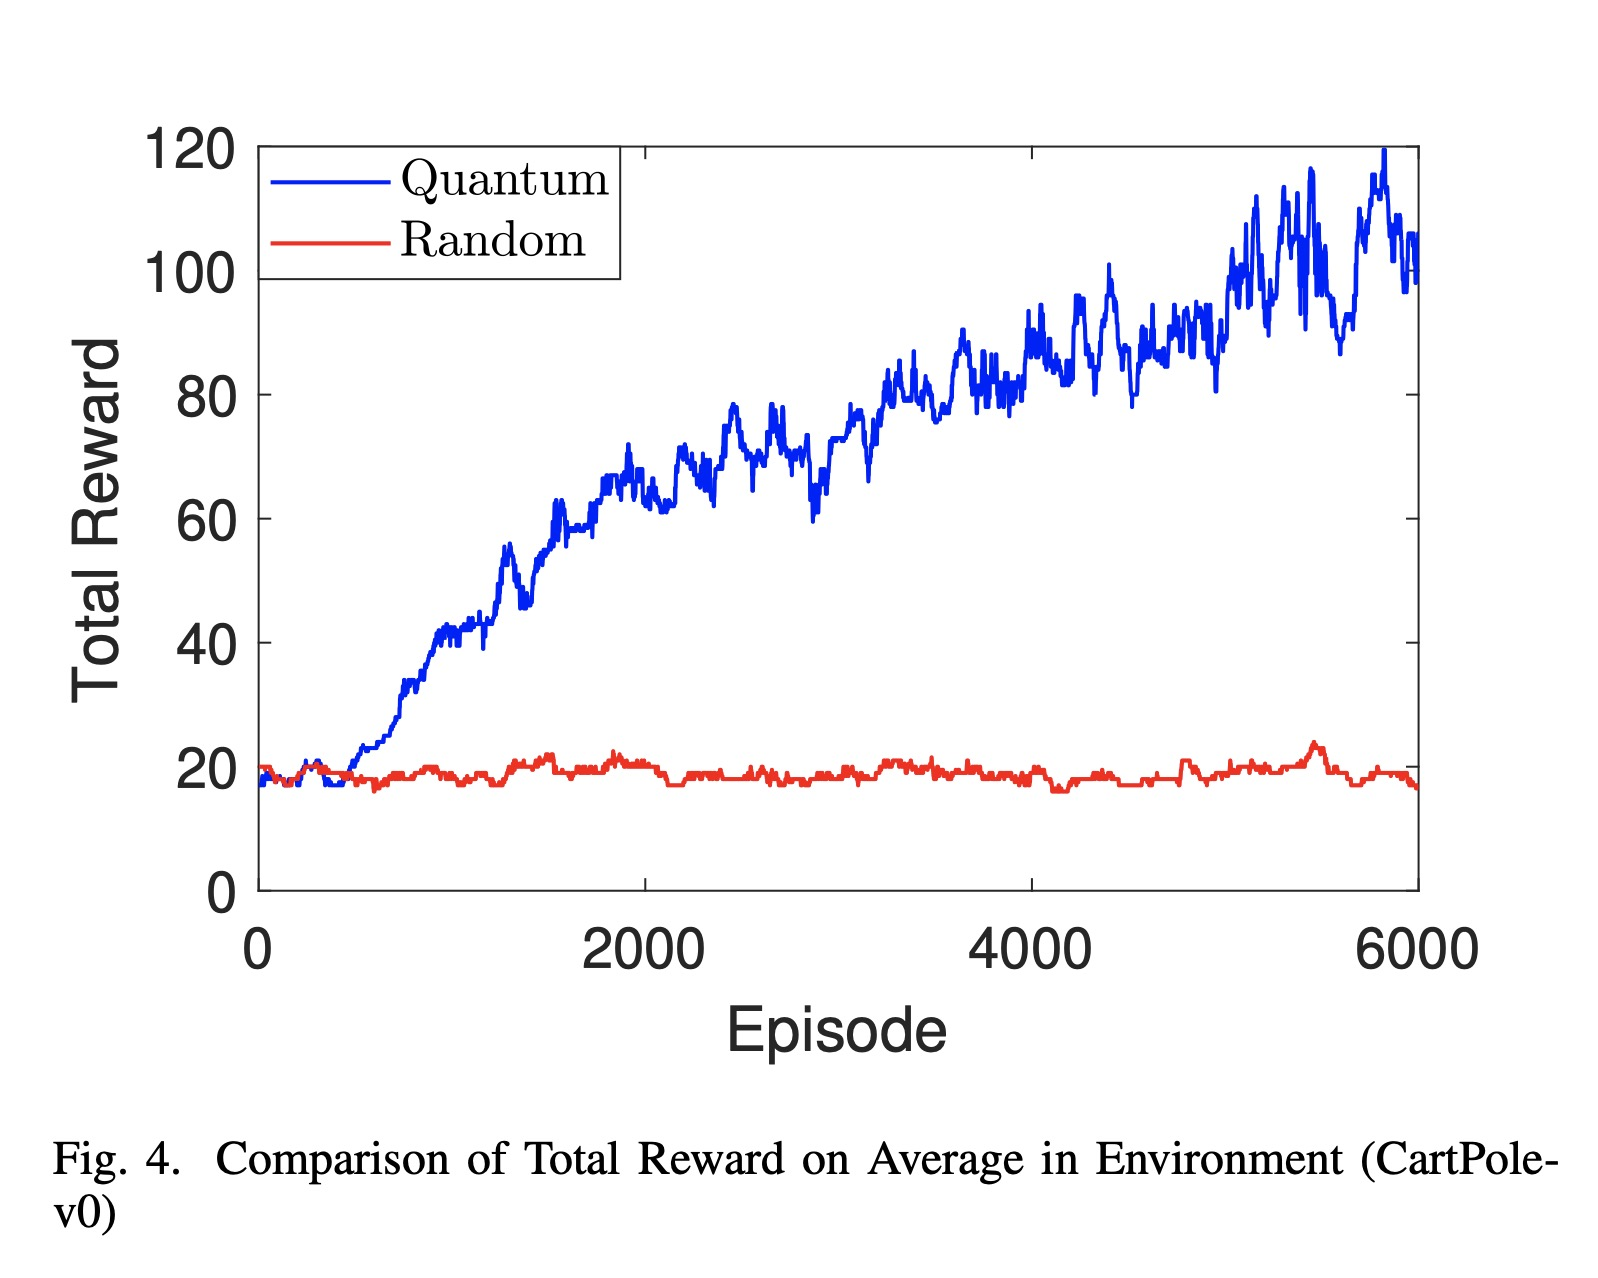
\includegraphics[scale=0.3]{tex/5.4.5_RL/result_paper.jpg}
  \caption{\label{stochastic} Comparison between RL and randomized strategy.}
\end{figure}


\subsection{Quantum Singular Value Decomposition}
\subsubsection{Background}
\paragraph{Singular Value Decomposition}
Singular Value Decomposition (SVD) is an important matrix decomposition in linear algebra. As a generalization of feature decomposition on arbitrary dimensional matrices, SVD is widely used in the field of machine learning, including matrix compression, recommendation systems, and natural language processing. It is defined as follows:
Given a complex matrix $M \in \mathbb{C}^{m \times n}$, define the SVD of the matrix $M$ as $M = UDV^\dagger$. Where $U$ is an $m \times m$ matrix, $V$ is an $n \times n$ matrix, and both $U$ and $V$ are unitary matrices, that is, satisfy $UU^\dagger = I$, $VV^\dagger = I$. $D$ is a diagonal matrix $m \times n$, with the elements of the main diagonal arranged from largest to smallest, and each element is called a singular value of the matrix $M$. 

\paragraph{Variational Quantum Singular Value Decomposition}
Quantum algorithms for SVD have been proposed in \cite{kerenidis2016quantum, rebentrost2018quantum}, which leads to applications in solving linear systems of equations \cite{wossnig2018quantum} and developing quantum recommendation systems \cite{kerenidis2016quantum}. However, these algorithms above are too costly to be convincingly validated for near-term quantum devices. The leading strategy to solve various problems using noisy intermediate-scale quantum (NISQ) devices are called variational quantum algorithms. 

\cite{wang2021variational} propose a variational quantum algorithm for singular value decomposition (VQSVD), formulating the task of SVD as an optimization problem. The detailed VQSVD algorithm is as follows: 
\begin{enumerate}
    \item Prepare the input of VQSVD algorithm: 
        \begin{itemize}
            \item A decomposition of the matrix $M$ into a linear combination of $K$ unitaries of the form $M = \sum_{k=1}^K c_k A_k$ with real numbers $c_k$. 
            \item Positive weights $q_1 > \cdots > q_r > 0$. 
            \item Computational basis {$\ket{\psi_1}, \cdots, \ket{\psi_T}$}, where $T$ is the desired rank. 
            \item Parameterized circuits $U(\theta)$, $V(\phi)$ with initial parameters of $\theta, \phi$. 
        \end{itemize}
    \item Enter a hybrid quantum-classical optimization loop to train the parameters $\theta$ and $\phi$ in the parameterized quantum circuits $U(\theta)$ and $V(\phi)$, compute the singular values of $M$: $m_j = \text{Re}\langle\psi_j|U(\theta)^{\dagger} M V(\phi)\ket{\psi_j}$. The goal is to maximum the designed loss $L(\theta, \phi)$: 
    \begin{equation}
        L(\theta, \phi) = \sum_{j=1}^T q_j \times \text{Re} \langle\psi_j| U(\theta)^{\dagger} M V(\phi)\ket{\psi_j}
    \end{equation}
    Where weights are added to make the calculated singular values descending. 
    \item Obtain optimal parameters $\alpha^ \star$ and $\beta^\star$ and compute $U(\alpha^\star)$ and $V(\beta^\star)$. 
    \item Obtain approximate singular values ${m_1, \cdots, m_r}$ and  singular vectors $U(\alpha^\star)$ and $V(\beta^\star)$. 
\end{enumerate}

\subsubsection{Application}
In this section, we show how to decompose a randomly generated $8 \times 8$ complex matrix using MindQuantum. 

First we need to introduce the required packages, define the required constants and set the weights, then use the $numpy.random.randint$ function to randomly generate an $8 \times 8$ complex matrix $M$:
\begin{lstlisting}
import os
os.environ['OMP_NUM_THREADS'] = '1'
from mindquantum import Simulator, MQAnsatzOnlyLayer, add_prefix
from mindquantum import Hamiltonian, Circuit, RY, RZ, X
import mindspore as ms
import numpy as np
from scipy.sparse import csr_matrix
from scipy.linalg import norm
from matplotlib import pyplot
import tqdm

n_qubits = 3  # qbits number
cir_depth = 20  # circuit depth
N = 2**n_qubits
rank = 8  # learning rank
step = 3
ITR = 200  # iterations
LR = 0.02  # learning rate

# Set equal learning weights
if step == 0:
    weight = ms.Tensor(np.ones(rank))
else:
    weight = ms.Tensor(np.arange(rank * step, 0, -step))

# Define random seed
np.random.seed(42)

def mat_generator():
    '''
    Generate a random complex matrix
    '''
    matrix = np.random.randint(
        10, size=(N, N)) + 1j * np.random.randint(10, size=(N, N))
    return matrix

# Generate matrix M which will be decomposed
M = mat_generator()
# m_copy is generated to error analysis
m_copy = np.copy(M)
print('Random matrix M is: ')
print(M)
# Get SVD results
U, D, v_dagger = np.linalg.svd(M, full_matrices=True)
\end{lstlisting}
Next define a hardware-efficient ansatz used in the simulation for $U(\theta)$ and $V(\phi)$, the variational ansatz used in the paper \cite{wang2021variational}. Since only real matrices are involved, the combination of rotation gates and CNOT is sufficient. In the ansatz, each same block(denoted in the dashed-line box) consists of a column of single-qubit rotations about the y-axis and z-axis following by a layer of CNOT gates which only connects the adjacent qubits. 
\begin{lstlisting}
class Ansatz:
    def __init__(self, n, depth):
        self.circ = Circuit()
        num = 0
        for _ in range(depth):
            for i in range(n):
                self.circ += RY('theta' + str(num)).on(i)
                num += 1
            for i in range(n):
                self.circ += RZ('theta' + str(num)).on(i)
                num += 1
            for i in range(n - 1):
                self.circ += X.on(i + 1, i)
            self.circ += X.on(0, n - 1)
\end{lstlisting}
Then define a quantum network using the given hamiltonian. The $set_q$ function of the simulator is used to set the state of the simulator to the given computational basis, so that we can obtain the measurement results under the basis, that is, the corresponding singular values. The $get\_expectation\_with\_grad$ function is used to compute the gradient of the parameters in the circuit and the value of the following expression: $E(\theta) = \langle\phi| U_l^{\dagger}(\theta) H U_r(\theta)\ket{\psi}$. Then we can use $MQAnsatzOnlyLayer$ to build a quantum network layer based on a given basis, and its output is: $\text{Re}\langle\psi_j|U(\theta)^{\dagger} M V(\phi)\ket{\psi_j}$. 
\begin{lstlisting}
def quantnet(qubits_num, hams, circ_right, circ_left=None, base=None):
    sim = Simulator('projectq', qubits_num)
    if base is None:
        pass
    else:
        sim.set_qs(base)
    grad_ops = sim.get_expectation_with_grad(hams, circ_right, circ_left)

    ms.context.set_context(mode=ms.context.PYNATIVE_MODE, device_target="CPU")
    quantumnet = MQAnsatzOnlyLayer(grad_ops, 'ones')
    return quantumnet
\end{lstlisting}
After sparring the decomposed $8 \times 8$ matrix $M$ and generating the corresponding Hamiltonian $H$, we can then instantiate ansatz $U_ansatz$ and $V_ansatz$ and build a required quantum network layer, which can be used to compute $\{m_j\}_{j=1}^T$, the singular values of $M$. 
\begin{lstlisting}
u_ansatz = add_prefix(Ansatz(n_qubits, cir_depth).circ, 'u')
v_ansatz = add_prefix(Ansatz(n_qubits, cir_depth).circ, 'v')
ham = Hamiltonian(csr_matrix(M))
i_matrix = np.identity(N)
quantum_models = dict()
quantum_models['net_0'] = quantnet(n_qubits, ham, v_ansatz, u_ansatz, i_matrix[0])
for s in range(1, rank):
    quantum_models["net_" + str(s)] = quantnet(n_qubits, ham, v_ansatz, u_ansatz, i_matrix[s])
    quantum_models["net_" + str(s)].weight = quantum_models['net_0'].weight
\end{lstlisting}
Additionally, we can use MindSpore to build a hybrid quantum-classical network to realize weighted summation of quantum network layers and compute $L(\theta,\phi) = \sum_{j=1}^T q_j \times \text{Re} \langle\psi_j| U(\theta)^{\dagger} M V(\phi)\ket{\psi_j}$. 
\begin{lstlisting}
class MyNet(ms.nn.Cell):
    '''
    define quantum-classic net
    '''
    def __init__(self):
        super(MyNet, self).__init__()

        self.build_block = ms.nn.CellList()
        for j in range(rank):
            self.build_block.append(quantum_models["net_" + str(j)])

    def construct(self):
        x = self.build_block[0]() * weight[0]
        k = 1
        for layer in self.build_block[1:]:
            x += layer() * weight[k]
            k += 1
        return -x
\end{lstlisting}
Now we can instantiate the hybrid quantum-classical network and start training using MindSpore: 
\begin{lstlisting}
net = MyNet()
# Define optimizer
opt = ms.nn.Adam(net.trainable_params(), learning_rate=LR)
# Simple gradient descent
train_net = ms.nn.TrainOneStepCell(net, opt)
# Start training
loss_list = list()
for itr in tqdm.tqdm(range(ITR)):
    res = train_net()
    loss_list.append(res.asnumpy().tolist())
\end{lstlisting}
Finally read the training results (the singular values) and compare them with the results of the classical singular value decomposition:
\begin{lstlisting}
singular_value = list()
for _, qnet in quantum_models.items():
    singular_value.append(qnet().asnumpy()[0])

print('Predicted singular values from large to small:', singular_value)
print("True singular values from large to small:", D)
\end{lstlisting}
Output:
\begin{lstlisting}
Predicted singular values from large to small: [54.83174, 19.169168, 14.88653, 11.093878, 10.533753, 7.648352, 5.5560594, -0.3320913]
True singular values from large to small: [54.83484985 19.18141073 14.98866247 11.61419557 10.15927045  7.60223249 5.81040539  3.30116001]
\end{lstlisting}
Intuitively, we can see that the singular values learned by using the hybrid quantum-classical network are similar to the real singular values. 




% \section{QuPack: Acceleration Engine}
% qupack简介

设计理念

与mq的关系

使用方法


% \subsection{Variational Quantum Eigensolver}
% 设计原理:粒子数和自选数守恒

性能与优势:
1. 简单罗列数据,比mq快多少
2. 强调对内存的压缩能力

% \subsection{Quantum Approximate Optimization Algorithm}
% 设计原理:ZZ哈密顿量绝热近似加速

性能与优势


% \subsection{Tensor Network Simulator}
% 介绍技术细节


% \subsection{Pulse Engineering}
% 介绍使用方法


% \section{Benchmarking}
% 场景:
1. 随机线路
2. 变分算法:qaoa,vqe(端到端)

数据集:
1. qaoa:4-ragular、全连通
2. vqe:氢链

框架:qulacs、qiskit、projectq、Intel-QS、QuEST、qupack、mindquantum

硬件:CPU、GPU、鲲鹏


% \section{Execution on Quantum Chip}

% \subsection{Circuit Compilation and Optimization}
% \begin{lstlisting}
mq中的编译框架:
1. DAG图
2. 如何通过小编译规则生成通用编译规则

现有规则

流程图
\end{lstlisting}


% \subsection{Qubit Mapping}
% 分工:朱祎康

介绍sabre算法

介绍使用方法

不足和要求:
如:必须要连通图


% \subsection{Quantum Virtual Machine}
% 设计原理:mq中如何基于噪声模拟、线路编译、比特映射完成芯片仿真任务

介绍定义好的QVM

% \subsection{Third-party Quantum Chip}
% 使用方法:如何连接真机运行

实例



% \section{Advanced Quantum Aplications}
% \subsection{CD QAOA}


%To run this example, follow the link

\subsubsection{Background}
In the field of quantum computing, researchers are continuously seeking efficient and robust methods to tackle complex problems. Adiabatic quantum computation (AQC) is one such approach, where a quantum system evolves gradually from an initial Hamiltonian to a final Hamiltonian that encodes the desired solution. According to the adiabatic theorem, if this evolution is slow enough, the system will remain in the ground state of the Hamiltonian throughout the process:

\begin{equation}
H(t) = (1-\lambda(t))H_{\text{initial}} + \lambda(t)H_{\text{final}},
\end{equation}

where $\lambda(t)\in[0,1]$. However, implementing AQC in practical scenarios faces challenges arising from external noise, imperfections, and the need for long evolution times. To overcome these limitations and enhance the efficiency of adiabatic evolution, one promising approach to solve this problem is the Quantum Approximate Optimization Algorithm (QAOA), where a parameterized quantum circuit (ansatz) prepares a trial state to approximate solutions for optimization problems. By optimizing the ansatz parameters, QAOA seeks to find the optimal values that minimize or maximize the objective function, which encodes the problem's energy landscape.

However, practical implementations of QAOA face challenges due to noise, decoherence, and the complexity of parameter optimization. To enhance its performance and robustness, the Counterdiabatic Quantum Approximate Optimization Algorithm (CD-QAOA) introduced the counterdiabatic (CD) term:
\begin{equation}
H_{\text{CD-QAOA}} = (1 - \lambda(t))H_{\text{initial}} + \lambda(t)H_{\text{final}} + H_{\text{CD}},
\end{equation}
It combines ideas from both AQC and the Quantum Approximate Optimization Algorithm (QAOA) by introducing one additional parameter per layer compared to QAOA. This results in shallower quantum circuits without compromising accuracy:
\begin{equation}
U(\gamma, \beta)\to U(\gamma, \beta, \alpha), \quad F(\gamma, \beta)\to F(\gamma, \beta, \alpha),
\end{equation}
where $\alpha, \beta, \gamma$ represents the digitized parameters, $F$ is cost function and $U$ is evolution operator..
The CD term acts as an extra component in the Hamiltonian and is carefully designed based on the instantaneous eigenstates and eigenenergies of the evolving Hamiltonian.  The counterdiabatic term effectively suppresses errors and reduces the required evolution time, leading to enhanced efficiency and reliability in quantum computations.

To derive the precise form of the counterdiabatic term, various techniques, such as Lewis-Riesenfeld invariants and transitionless quantum driving, have been applied. The implementation of the CD term is tailored to the specific problem and dynamics of the quantum system, utilizing available control techniques. In cases where obtaining exact CD terms becomes challenging, an approximate CD driving approach is proposed, utilizing the nested commutator method\cite{Chandarana_2023} with the adiabatic gauge potential:

\begin{equation}
A_{\lambda}^{(l)} = i\sum_{k=1}^{l}\alpha_{k}(t)[H_{a},[H_{a},...[H_{a}, \partial_{\lambda}H_{a}]]].
\end{equation}

DC-QAOA holds promise for solving a wide range of optimization problems, from combinatorial optimization to machine learning tasks and financial portfolio optimization. As quantum computing technology continues to advance, DC-QAOA represents an exciting avenue for leveraging the counterdiabatic term and parameter space digitization to unlock new frontiers in quantum optimization.

\textbf{Target problem}
\begin{itemize}
\item[1.] Learn how to find the ground state of problem Hamiltonian
\item[2.] Utilize quantum circuits to find optimized parameters 
\end{itemize}
\textbf{Required Mindquantum functionalities}
\begin{itemize}
\item[1.] gradient-based optimizer
\item[2.] Batch quantum circuit simulator

\end{itemize}

\subsubsection{Implement}
As a mature application of QAOA, this algorithm requires two steps, which is building the ansatz circuit and optimization. Now let's look at how to implement Digitized-counterdiabatic quantum approximate optimization algorithm (DC-QAOA) into Ising spin model, the model is depicted in Fig.~\ref{fig:ising}. The initial state is choose as $H_{initial} = \sum_{i}\sigma_{i}^{x}$. The general form of the Hamiltonian of the 1D Ising spin model is given by
\begin{figure}
    \centering
    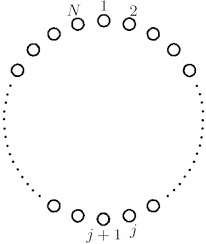
\includegraphics[width=0.5\linewidth]{5.4.1_figure/ising.jpg}
    \caption{Schematic picture of the Ising model}
    \label{fig:ising}
\end{figure}

\begin{equation}
H_{final} = -\sum_{\langle i,j \rangle}J_{ij}\sigma_{i}^{z}\sigma_{j}^{z} - \sum_{i}h_{i}\sigma_{i}^{z} - \sum_{i}k_{i}\sigma_{i}^{x}.
\end{equation}
\begin{lstlisting}
# generate H_{initial} as H_{mixer}
# n_qubits is the number of qubits
def generate_h_mixer(n_qubits:int):
    h_mixer = QubitOperator()
    for i in range(n_qubits):
        h_mixer += QubitOperator(f'X{i}')
    return h_mixer
    
# generate H_{final} as H_{prob}
def generate_h_prob(n_qubits:int, J:float, h:float, k:float):
    h_prob = QubitOperator()
    for i in range(n_qubits):
        j = (i+1)%n_qubits
        h_prob += QubitOperator(f'Z{i} Z{j}', J)
        h_prob -= QubitOperator(f'Z{i}', h)
        h_prob -= QubitOperator(f'X{i}', k)
    return h_prob
\end{lstlisting}

In our case,  a pool of CD operators is defined using the nested commutator approach of the adiabatic gauge potential \cite{PhysRevResearch.4.013141}
$$A = \{\sigma^{y},\sigma^{z}\sigma^{y}, \sigma^{y}\sigma^{z}, \sigma^{x}\sigma^{y}, \sigma^{y}\sigma^{x} \}.$$

Here we present a 12 qubits system and we consider second-order $A = \sum_{i}\sigma_{i}^{z}\sigma_{i+1}^{y}$. For simplify, we choice  $J = -1, h = 0, k = -1$. Following we build an ansatz layer for DC-QAOA.
\begin{lstlisting}
def generate_h_cd(n_qubits:int):
    h_cd = QubitOperator()
    for i in range(n_qubits-1):
        h_cd += QubitOperator(f'Z{i} Y{i+1}')
    return h_cd
\end{lstlisting}    

\begin{lstlisting}
n_qubits = 12
J, h, k = -1, 0, -1

h_prob = generate_h_prob(n_qubits, J, h, k)
h_mixer = generate_h_mixer(n_qubits)
h_cd = generate_h_cd(n_qubits)
\end{lstlisting}

In order to prepare the eigenstate for $H_{initial}$, we first put ${\rm prep\_circ}$, and then apply evolution operator on it. 
\begin{lstlisting}
# generate the eigenstate for $H_{mixer}$
prep_circ = UN(H, n_qubits)

# choose two layer 
p = 3
ansatz_template = u_p + u_m + u_cd

ansatz = Circuit() + prep_circ
for i in range(p):
    ansatz += add_suffix(ansatz_template, str(i)) + BarrierGate()
\end{lstlisting}

As long as we have set up the ansatz circuit, we can change the number of layers or type of optimizer in order to find the optimal parameter set. We define cost function using 
\begin{equation}
E = \left<\psi_0\right|U^{\dagger}\ H_{prob} U\left|\psi_0\right>,
\end{equation}
where $U = \Pi_{i=0}^3 U_{cd}(\alpha_i)U_m(\beta_i)U_p(\gamma_i)$ and this is just the evolution operator. 
\begin{lstlisting}
energys = []
# define cost function
def fun(x0, grad_ops, energys):
    f, g = grad_ops(np.array(x0))
    f = np.real(f[0, 0])
    g = np.real(g[0, 0])
    energys.append(f)
    if len(energys)%5==0:
        print(f"step: {len(energys)}, energy: {f}")
    return f, g
\end{lstlisting}

In this tutorial, we will optimize the gradient using BFGS optimizer\cite{chandarana2022meta}, which will have good enough results. If you plot the figure of mean energy, you will have result like Fig.~\ref{fig:dc}. Here, the green line is the exact eigenvalue of $H_{prob}$, the blue line is the mean value during the optimizing process, the orange line is QAOA with three layers. We can notice that DC-QAOA  has converged to the exact value in 70 steps within 0.5s. Comparing these two algorithm from the ability of estimating the ground state, DC has advantage over QAOA.
\begin{figure}
    \centering
    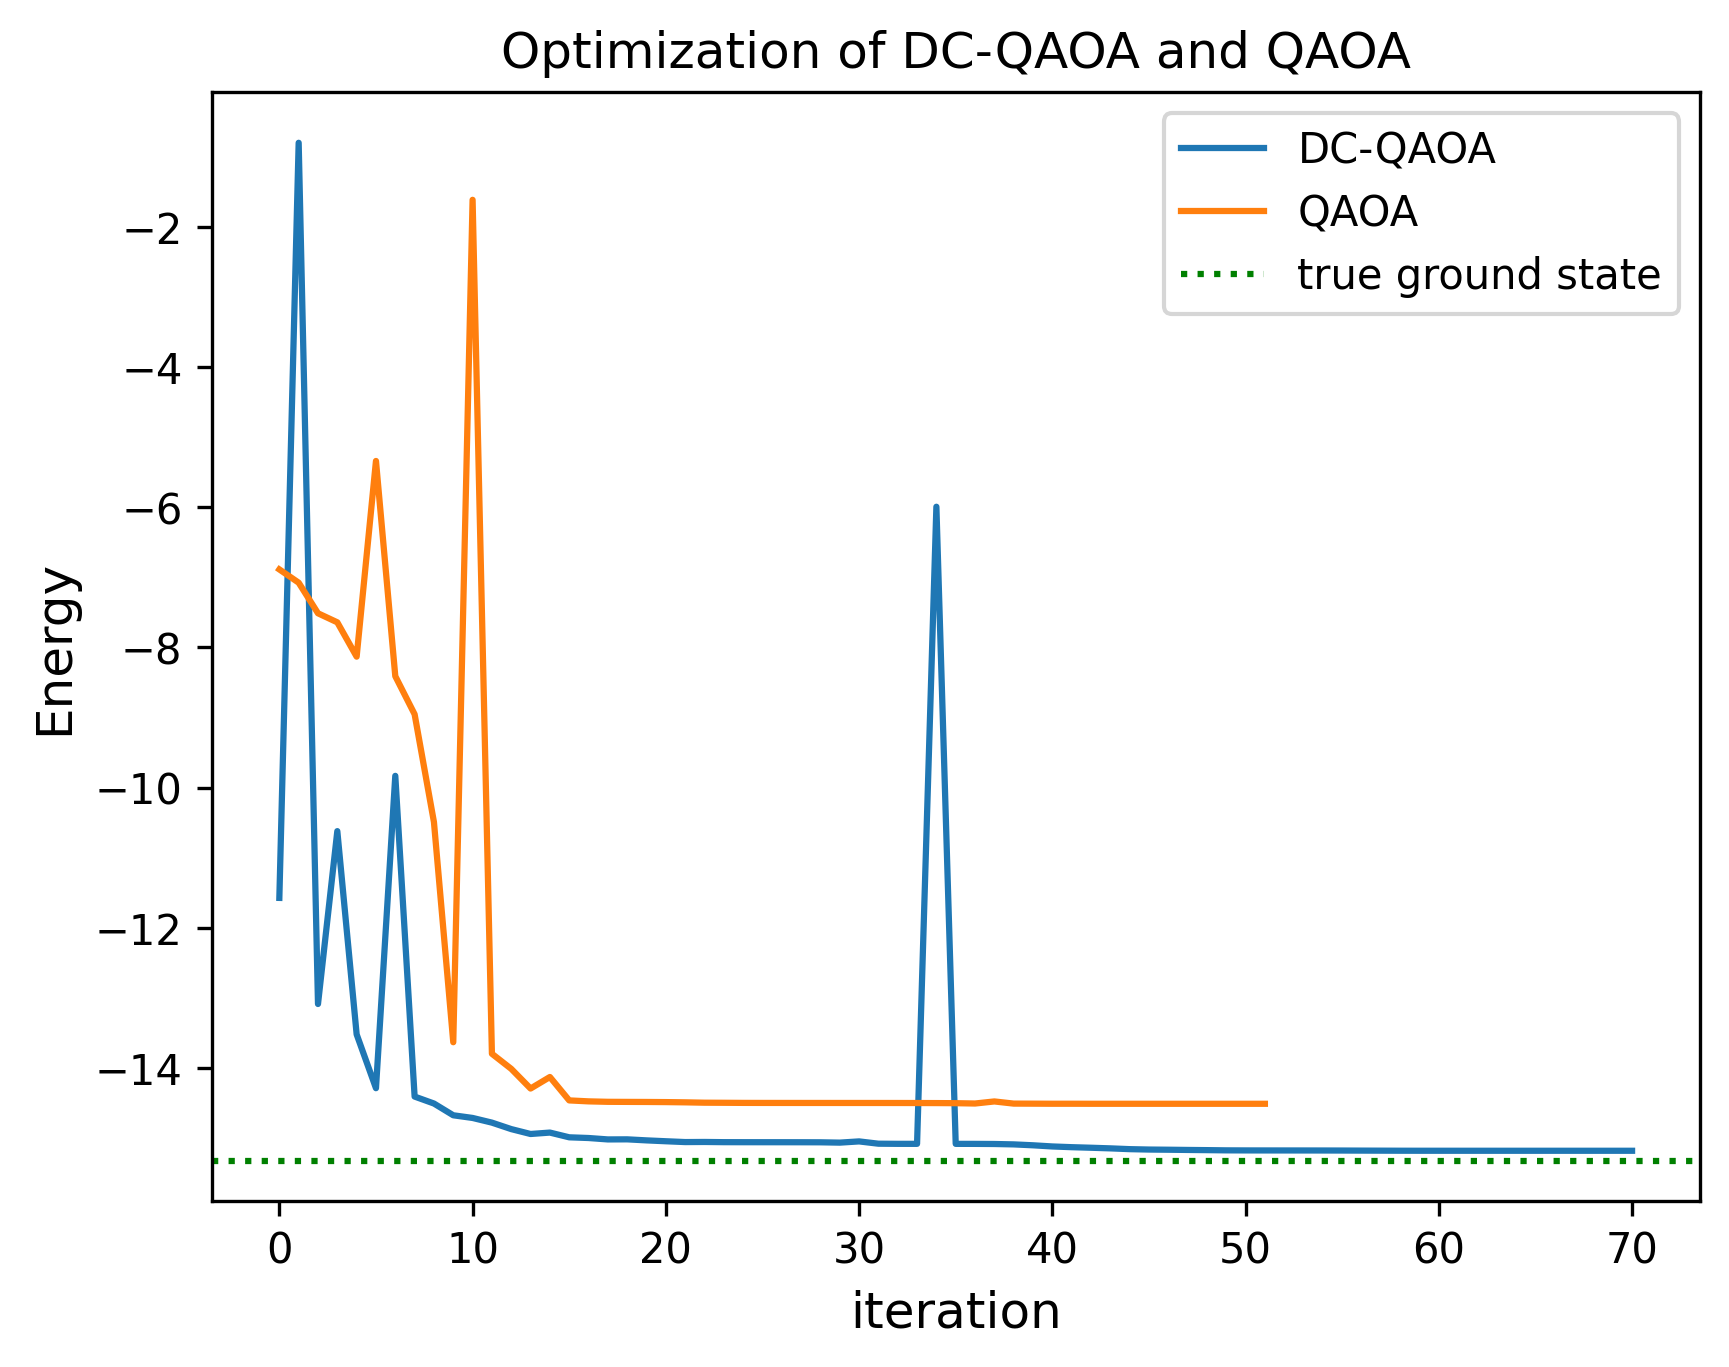
\includegraphics[width = 1 \linewidth]{5.4.1_figure/DC-WHITE.png}
    \caption{Mean Energy vs. iteration time}
    \label{fig:dc}
\end{figure}





\subsection{Symmetry enhanced VQE}
The study of variational quantum algorithms has largely been focused on identifying the ground state of intricate many-body systems. In this context, the Variational Quantum Eigensolver (VQE) algorithm has emerged as a potent tool, designed to target the ground state of a many-body system by minimizing average energy. However, several critical phenomena in physics, including topological phases, necessitate knowledge of several low-energy eigenstates, not just the ground state. Therefore, the generalization of VQE to higher energy eigenstates is highly important.

The weighted SSVQE provides an alternative method to generate all the $k$ lowest energy eigenstates of a given Hamiltonian $H$~\cite{?}. This method utilizes a set of $k$ orthogonal initial states, denoted as $\{|\phi_{i}\rangle\}_{i=1}^{k}$ (where $\langle \phi_{i} | \phi_{j} \rangle = \delta_{ij}$), as the input of a single parameterized quantum circuit, described by the unitary operator $U(\vec{\theta})$. Given that the initial states are orthogonal, the outputs $U(\vec{\theta})| \phi_{j} \rangle$, generated by the same circuit, maintain orthogonality. In the weighted SSVQE, the objective is to minimize the cost function
\begin{equation}
    \mathrm{cost} = \sum_{i=1}^{k} w_{i} \langle \phi_{i}| U^{\dagger}(\vec{\theta}) H U(\vec{\theta}) | \phi_{i} \rangle
    \label{ssvqe_cost}
\end{equation}
where $w_1 > w_2 > \cdots > w_k$ are real positive numbers. Minimizing the cost function in Eq.~\eqref{ssvqe_cost} produces all the $k$ lowest energy eigenstates such that $|E_{i}\rangle = U(\vec{\theta}^{*})|\phi_{i}\rangle$.
A notable advantage of the weighted SSVQE is that it delivers all the $k$ lowest energy eigenstates through a single optimization process, without requiring any overlap of quantum states. However, the algorithm becomes more resource-demanding as the number of target eigenstates increases.

Symmetry is one of the most profound concepts in physics, especially in quantum mechanics. A majority of physical systems exhibit various types of symmetries that can be accurately described mathematically. The VQE algorithm can also significantly benefit from the integration of these symmetries. There are two ways to incorporate symmetries in the VQE algorithms: (i) designing the circuit to naturally generate the quantum states with the relevant symmetry~\cite{?}, and (ii) adding extra terms to the cost function to penalize the quantum states without the relevant symmetry~\cite{?}.


Leveraging the adaptability and comprehensive capabilities of MindQuantum, researchers are able to work with any optimization target by defining custom objective functions. Here, we present an example of implementing SSVQE through MindQuantum to accurately determine the four lowest state energies of the Heisenberg Hamiltonian, employing different symmetry incorporation strategies.


The full notebook and implementation is available at:
XXXXXXXXX

First, we need to construct the symmetry preserving ansatz~\cite{?}.
\begin{lstlisting}
def entangling_gate(parameter, qubits):
    circuit = Circuit()
    circuit += RZ(-np.pi / 2).on(qubits[1])
    circuit += CNOT.on(qubits[0], qubits[1])
    circuit += RZ({parameter: -2}).on(qubits[0])
    circuit += RZ(np.pi / 2).on(qubits[0])
    circuit += RY({parameter: 2}).on(qubits[1])
    circuit += RY(-np.pi / 2).on(qubits[1])
    circuit += CNOT.on(qubits[1], qubits[0])
    circuit += RY({parameter: -2}).on(qubits[1])
    circuit += RY(np.pi / 2).on(qubits[1])
    circuit += CNOT.on(qubits[0], qubits[1])
    circuit += RZ(np.pi / 2).on(qubits[0])
    return circuit

def ansatz(N, layers, local_rot=True):
    circuit = Circuit()
    params_index = 0
    for layer_index in range(layers):
        for i in range(2):
            for j in range(i, N - 1, 2):
                circuit += entangling_gate(str(params_index), [j, j + 1])
                params_index += 1
        if local_rot:
            for i in range(N):
                circuit += PhaseShift(params_index).on(i)
                params_index += 1
    return circuit
\end{lstlisting}

The SSVQE can then be implemented as a combination of several VQEs with distinct initialization circuits yet utilizing a shared parameter ansatz. One need to ensured that the resulting states post-initialization are orthogonal.
For each VQE, a unique measurement function can be defined to accomplish a variety of tasks.
Using the "get\_expectation\_with\_grad" function, one can easily obtain the expectation value and the corresponding gradient with respect to the trainable variables. Here, as an example, we demonstrate the code implementation for obtaining the second and the third lowest state energies of the Heisenberg Hamiltonian. In this particular instance,
we use a $S_z$-conserving ansatz, which preserves the $z$ component of the total spin, and the total spin operator is added to the cost function as a penalty term. The cost function is then modified into a form of
\begin{equation}
    \mathrm{cost} = \sum_{i=1}^{k} w_{i} \langle \phi_{i}| U^{\dagger}(\vec{\theta}) [H + (\hat{O} - c)^2] U(\vec{\theta}) | \phi_{i} \rangle,
    \label{ssvqe_cost_pen}
\end{equation}
where $c$ is a constant indicating the target subspace. Here, we do the expansion $(\hat{O} - c)^2 {=} \hat{O}^2 {-} c\hat{O} {+} c^2$. Together with the Hamiltonian, now we have three different measurement operators.

\begin{lstlisting}
class SSVQE:
    def __init__(self, n_qubits, init_circuits, pqc, ops):
        self.n_qubits = self.n_qubits
        self.circs = [circ + pqc for circ in init_circuits]
        self.sim = Simulator('mqvector', n_qubits)
        self.grad_ops = [self.sim.get_expectation_with_grad(ops, circ) for circ in circs]
    
    def __call__(self, inputs):
        cost = 0
        cost_grad = 0
        for i in range(len(self.grad_ops)):
            f, g = self.grad_ops[i](inputs)
            f1, f2, f3 = f[0, 0].real, f[0, 1].real, f[0, 2].real
            g1, g2, g3 = np.array(g[0, 0, :].real), np.array(g[0, 1, :].real), np.array(g[0, 2, :].real)
            cost += (f1 + f2 + f3) * (len(self.grad_ops) - i)
            cost_grad += (g1 + g2 + g3) * (len(self.grad_ops) - i)
        return cost, cost_grad
\end{lstlisting}

Now we need to set up the training function for the SSVQE. With all the module we predefined, the procedure is straightforward. The choice of the classical optimizer is flexible as well, here we choose the "L-BFGS-B" optimizer implemented in SciPy.

\begin{lstlisting}
def training(ssvqe, optimizer):
    initial_parameter = (np.random.rand(len(ssvqe.circs[0].params_name)) - .5) * np.pi
    result = optimizer.minimize(ssvqe, initial_parameter, jac=True, method='l-bfgs-b')
    return result
\end{lstlisting}

This implementation takes several minutes to finish training. One can track the results after each optimization step and generate a plot to compare the approximation results with the actual energies. In Fig.~\ref{}, we show the simulation results for the four lowest state energies of the Heisenberg Hamiltonian. It is clear to see that, incorporating SSVQE with the inherent symmetries, one can approximate both the ground and excited state energies precisely in a resource-efficient manner.

\subsection{Data-reuploading Classifier}
\input{5.4.3_Data-reuploading_Classifier}

\subsection{Q-GAN}
分工:舒润秋

\subsection{Reinforcement Learning}
\textit{Introduction} -- An overall reinforcement learning algorithm(RL) is composed of Agent, Environment, State, Action, and Reward. After the Agent executes an action, the Environment switches to a new State according to the Action and gives a Reward according to certain rules. After that, the Agent updates its decision-making process according to the obtained new State and Reward and gives a new Action, and so on, until the entire control process is completed. We denote $\pi_{\theta}$ as the policy function, $s$ as each state of the environment, $r$ as the reward in each state, and $a$ as the action of the agent. The architecture of RL is demonstrated in Figure~\ref{RL_frame}.
\begin{figure}[ht]
  \centering
  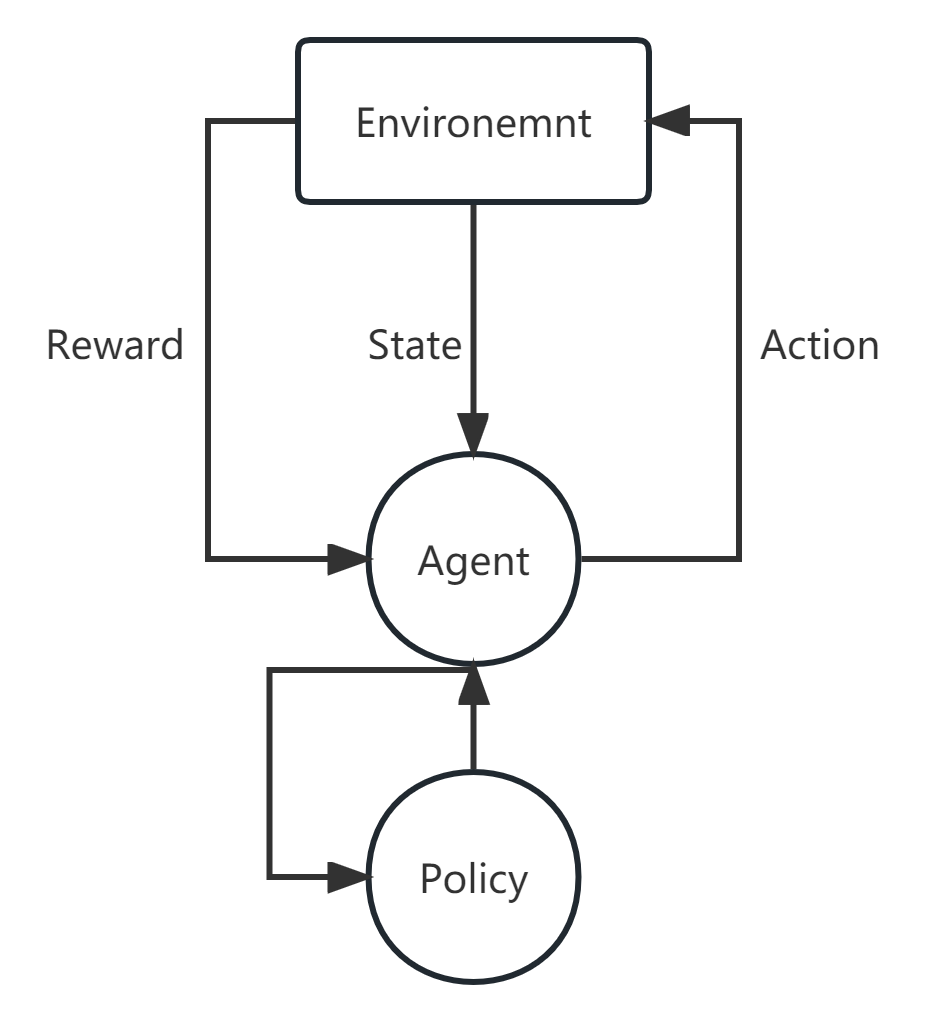
\includegraphics[scale=0.4]{tex/5.4.5_RL/RL.png}
  \caption{\label{RL_frame} The demonstration of RL wroking process.}
\end{figure} 

We assumed an environment has $N$ different states. And we act action $a_{i-1}$ on state $s_{i-1}$ with the result $s_{i}$. The transition probability function from state $s_{i-1}$ to state $s_{i}$ can be $P(s_{i+1}|s_{i},a_{i})$. Meanwhile, there is a reward $r_i$ in each state calculated by reward function $R_i=R(a_i,s_i,s_{i-1})$. In the progress of environmental change, the reward expectation is only determined by the latest $state$, which is called the Markov decision process. Therefore, each $T$ step trajectory will be chosen by the agent with probability:

\begin{equation}
    \begin{split}
        &P(\tau|\pi_{\theta})=\\
        &\rho(s_0)\prod_{k=0}^{k=T-1}P(s_{k+1}|s_{k},a_{k})\pi_{\theta}(a_{k}|s_{k})
    \end{split}
\end{equation}
where $\rho$ is the initial state distribution. Then the expectation of $T$ steps trajectory's reward is:
\begin{equation}
    \eta(\pi_{\theta})=\int_{\tau}P(\tau|\pi_{\theta})R(\tau)d\tau
\end{equation}
In order to get the optimal policy function $\pi_{\theta}$, the agent is trained to maximize the expectation $\eta$, which is:
\begin{equation}
    \pi_{\theta}^{opt}=\mathrm{argmax}_{\theta}\eta(\pi_{\theta})
\end{equation}
In following sections, we will demonstrate how to the agent in quantum devise.
\textit{Hybrid Deep Q-Network} -- Replace the neural network in the classical Deep Q-network's agent with the quantum variational circuit, we get the hybrid deep Q-network(HDQN)~\cite{Q_rl}. The architecture of HDQN is illustrated in FIG. We calculate the parameters $\theta$ by classical neural network and use them to construct the quantum variational circuit. Finally, the quantum part applies the action to the environment. Meanwhile, the environment responds with a reward $r_i$. We denote $e_i=(s_i,a_i,r_{i+1},s_{i+1})$ as a experience. In the training stage, we will use these experiences as training samples to adjust the parameters in both the classical part and quantum part according to loss function $L(\theta)$:
\begin{equation}
\begin{split}
    L(\theta_{j})=&E[R_{i+1}+\\
    &\gamma \max_{\alpha^{'}}Q(s_{i+1},a^{'},\theta_{j}^{-})-Q(s_{i},a_{i},\theta_{i})^2]
\end{split}
\label{loss func}
\end{equation}

\textit{Variational quantum circuit} -- The variational quantum circuit is a quantum circuit using adjustable parameters that can be changed by the external environment. Here, according to the architecture in ~\cite{Q_rl}, we construct the quantum circuit with the combination of encoder and ansatz. Here, we apply the Hardware Efficient circuit as the ansatz. The overall quantum circuit is illustrated in Figure~\ref{Agent_qc}.

\begin{figure*}[ht]
  \centering
  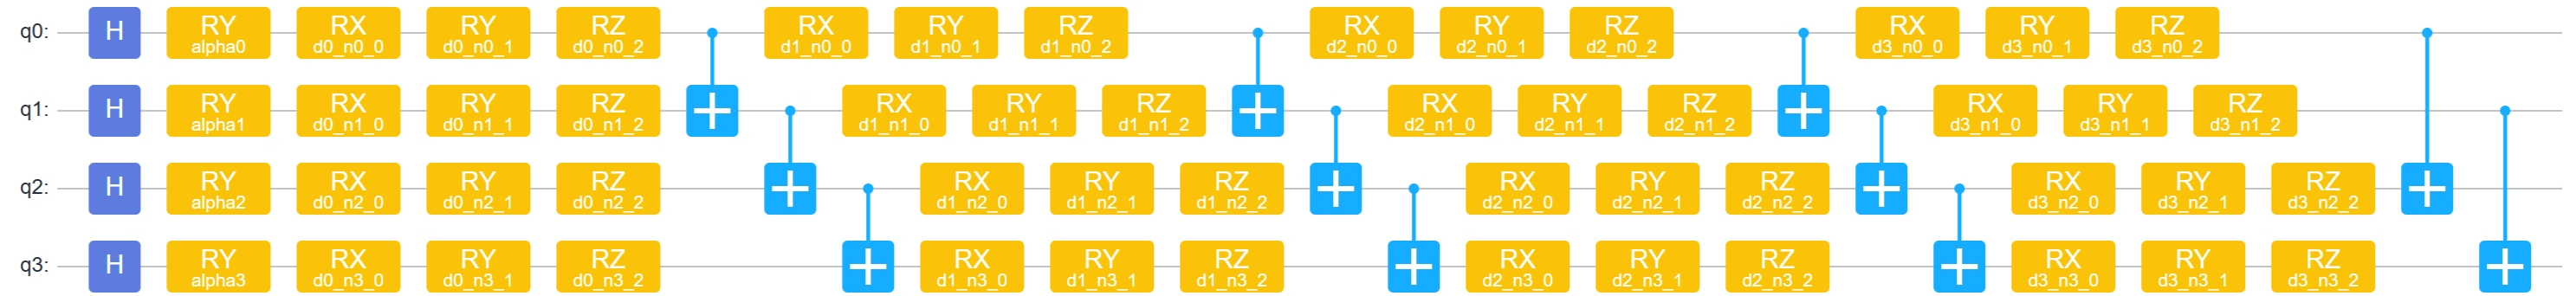
\includegraphics[scale=0.5]{tex/5.4.5_RL/Circuit.png}
  \caption{\label{Agent_qc} The overall quantum circuit of agent in RL.}
\end{figure*}

\textit{The implement in mindquantum} -- Here, we give the example of realizing HDQN by mindquantum. The first step is to construct the quantum variational circuit including the encoder and the ansatz.
\begin{lstlisting}
    def __get_encoder(self):
        encoder = Circuit()                                  
        encoder += UN(H, 4)                                  
        for i in range(4):                                   
            encoder += RY(f'alpha{i}').on(i)                  
        encoder = encoder.no_grad()                           
        quantum circuit which has no gradient: no_grad()
        encoder.summary()                                    
        return encoder
    def __get_ansatz(self):
        ansatz = HardwareEfficientAnsatz\\
            (4, single_rot_gate_seq=[RX,RY,RZ],\\
            entangle_gate=X, depth=3).circuit     
        ansatz += X.on(2,0)
        ansatz += X.on(3,1)
        ansatz.summary()                                                                              
        return ansatz
    self.circuit = self.encoder + self.ansatz
\end{lstlisting}

After the progress of the quantum circuit, we need to construct an observable Hamiltonian as a measurement basis. Here, we only measure the second and third qubits on $\sigma_y$ base. The Hamiltonian is as follows:
\begin{equation}
    H=I\otimes I\otimes\sigma_y\otimes\sigma_y
\end{equation}
We can construct the hamiltonian by mindquantum as follows:
\begin{lstlisting}
    def __get_observable(self):
        hams=[Hamiltonian(QubitOperator(f'Y{i}'))\\
            for i in [2, 3]] 
        return hams
\end{lstlisting}
Moreover, we can easily get the expectation and calculate the gradient of expectation by function $get\_expectation\_with\_grad$, which can be used to optimize parameters.

Next, we need to realize the classical part, which is a three-layers fully connected neural network with activation function Relu.
\begin{lstlisting}
    class Critic(nn.Cell):
        def __init__(self):
            super(Critic, self).__init__()
            self.relu = nn.ReLU()
            self.fc1 = nn.Dense(4, 64)
            self.fc2 = nn.Dense(64, 256)
            self.fc3 = nn.Dense(256, 1)
    
        def construct(self, x):
            x = self.relu(self.fc1(x))
            x = self.relu(self.fc2(x))
            x = self.fc3(x)
            return x
\end{lstlisting}

\textit{environment} -- Here, we focus on the problem of the gym game "CartPole-v0". It's a game that has an unbalanced cart on a track. This game has two inputs $0$ and $1$, which correspond to two directions left and right respectively. Users should control the trace moving toward these two directions and keep the cart balanced as long as possible.

The first step is to create the environment by gym.
\begin{lstlisting}
    import gym
    env = gym.make('CartPole-v0')
\end{lstlisting}
\textit{Memory buffer} -- In the progress of training, the training samples are randomly selected from the previous experience $e_i$. Therefore, we need to construct a buffer to store and sample the experience $e_i$.
\begin{lstlisting}
class Memory(object):
    ......
\end{lstlisting}
\textit{Training} -- The final step is model training. At first, we initialize HDQN with random parameters and let the actor interact with the environment. Next, we store the interaction result in the memory buffer as training samples. Finally, we sample from the memory buffer and adjust the parameters both in the classical part and quantum part with loss function (\ref{loss func}). Because of the space limitation, we will not provide the detailed code here.

\textit{Result of numerical simulation} -- In order to evaluate the result of the HDQN. We do some experiments to evaluate the performance. As shown in Figure ~\ref{stochastic} We compare the average results from multiple experiments with randomized strategy experiments. The results show that reinforcement learning using quantum circuits as the agent has indeed learned the strategy.
\begin{figure}[ht]
  \centering
  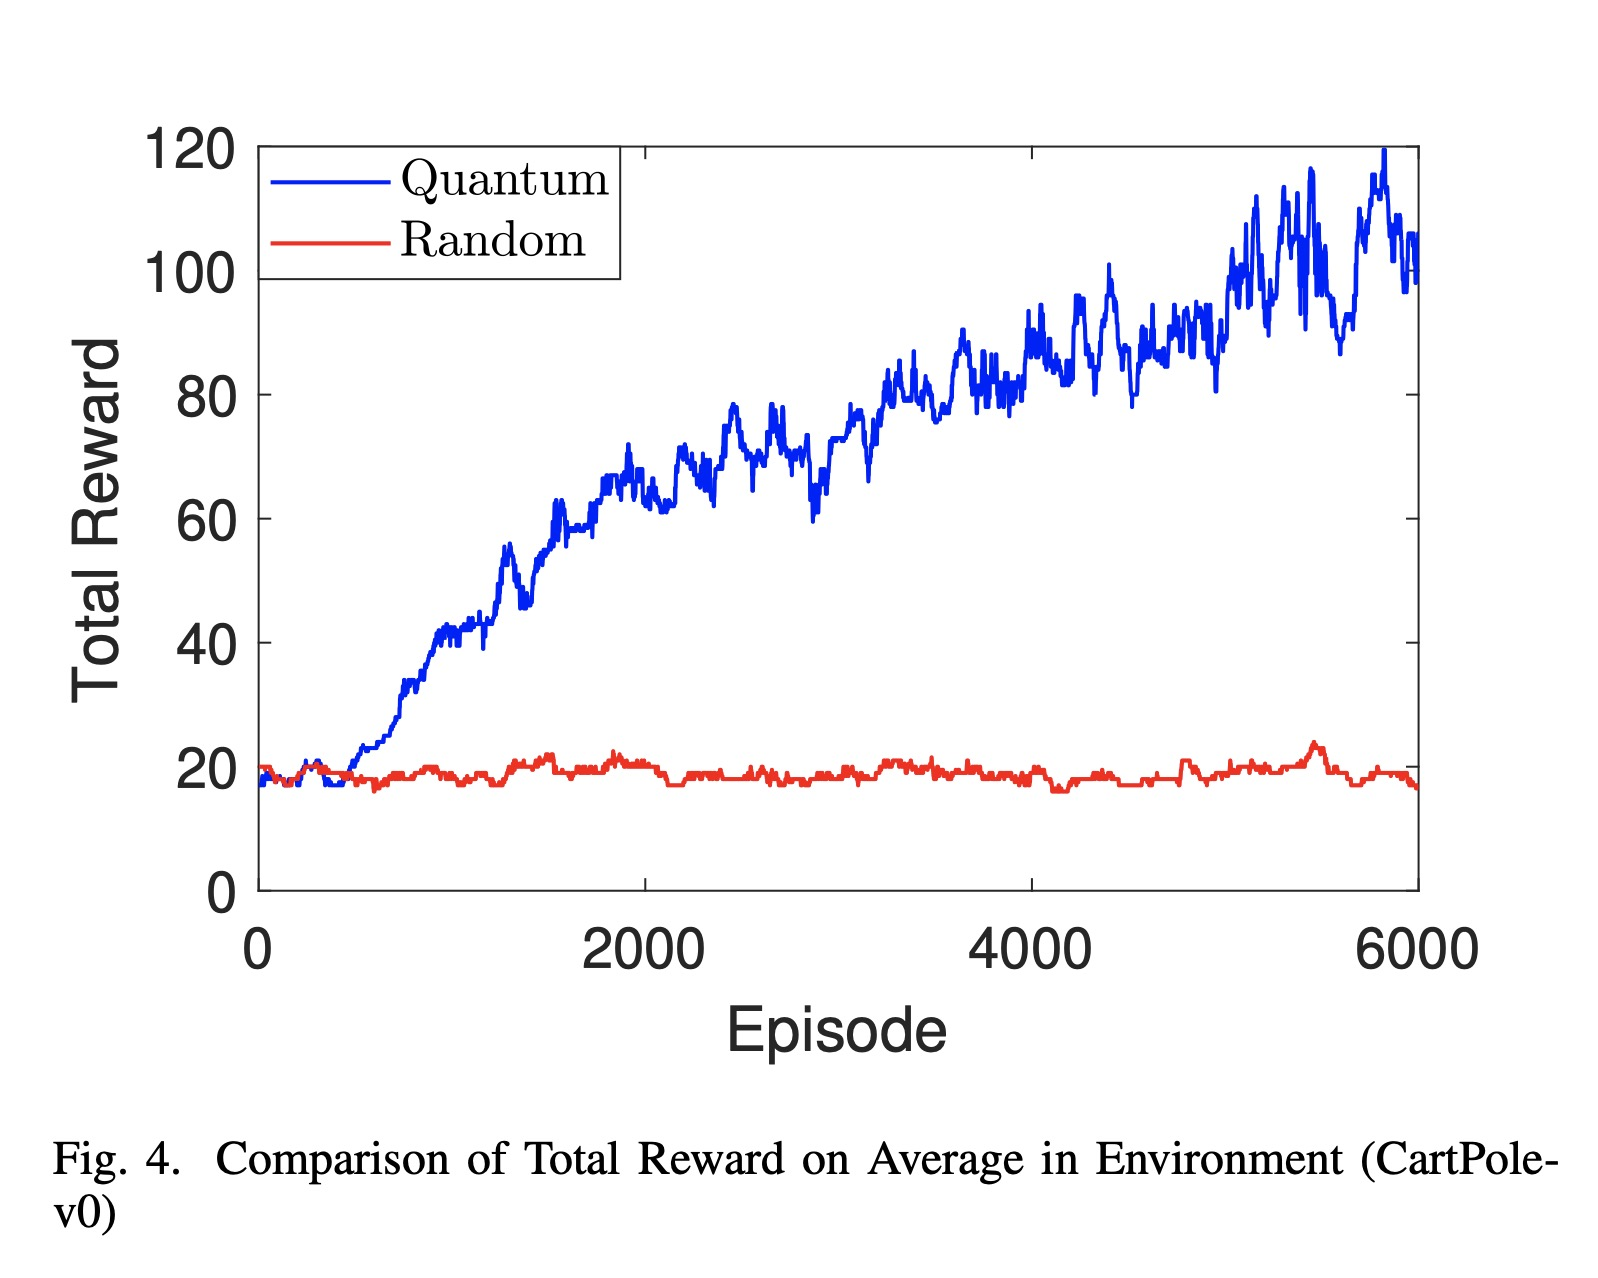
\includegraphics[scale=0.3]{tex/5.4.5_RL/result_paper.jpg}
  \caption{\label{stochastic} Comparison between RL and randomized strategy.}
\end{figure}


\subsection{Quantum Singular Value Decomposition}
\subsubsection{Background}
\paragraph{Singular Value Decomposition}
Singular Value Decomposition (SVD) is an important matrix decomposition in linear algebra. As a generalization of feature decomposition on arbitrary dimensional matrices, SVD is widely used in the field of machine learning, including matrix compression, recommendation systems, and natural language processing. It is defined as follows:
Given a complex matrix $M \in \mathbb{C}^{m \times n}$, define the SVD of the matrix $M$ as $M = UDV^\dagger$. Where $U$ is an $m \times m$ matrix, $V$ is an $n \times n$ matrix, and both $U$ and $V$ are unitary matrices, that is, satisfy $UU^\dagger = I$, $VV^\dagger = I$. $D$ is a diagonal matrix $m \times n$, with the elements of the main diagonal arranged from largest to smallest, and each element is called a singular value of the matrix $M$. 

\paragraph{Variational Quantum Singular Value Decomposition}
Quantum algorithms for SVD have been proposed in \cite{kerenidis2016quantum, rebentrost2018quantum}, which leads to applications in solving linear systems of equations \cite{wossnig2018quantum} and developing quantum recommendation systems \cite{kerenidis2016quantum}. However, these algorithms above are too costly to be convincingly validated for near-term quantum devices. The leading strategy to solve various problems using noisy intermediate-scale quantum (NISQ) devices are called variational quantum algorithms. 

\cite{wang2021variational} propose a variational quantum algorithm for singular value decomposition (VQSVD), formulating the task of SVD as an optimization problem. The detailed VQSVD algorithm is as follows: 
\begin{enumerate}
    \item Prepare the input of VQSVD algorithm: 
        \begin{itemize}
            \item A decomposition of the matrix $M$ into a linear combination of $K$ unitaries of the form $M = \sum_{k=1}^K c_k A_k$ with real numbers $c_k$. 
            \item Positive weights $q_1 > \cdots > q_r > 0$. 
            \item Computational basis {$\ket{\psi_1}, \cdots, \ket{\psi_T}$}, where $T$ is the desired rank. 
            \item Parameterized circuits $U(\theta)$, $V(\phi)$ with initial parameters of $\theta, \phi$. 
        \end{itemize}
    \item Enter a hybrid quantum-classical optimization loop to train the parameters $\theta$ and $\phi$ in the parameterized quantum circuits $U(\theta)$ and $V(\phi)$, compute the singular values of $M$: $m_j = \text{Re}\langle\psi_j|U(\theta)^{\dagger} M V(\phi)\ket{\psi_j}$. The goal is to maximum the designed loss $L(\theta, \phi)$: 
    \begin{equation}
        L(\theta, \phi) = \sum_{j=1}^T q_j \times \text{Re} \langle\psi_j| U(\theta)^{\dagger} M V(\phi)\ket{\psi_j}
    \end{equation}
    Where weights are added to make the calculated singular values descending. 
    \item Obtain optimal parameters $\alpha^ \star$ and $\beta^\star$ and compute $U(\alpha^\star)$ and $V(\beta^\star)$. 
    \item Obtain approximate singular values ${m_1, \cdots, m_r}$ and  singular vectors $U(\alpha^\star)$ and $V(\beta^\star)$. 
\end{enumerate}

\subsubsection{Application}
In this section, we show how to decompose a randomly generated $8 \times 8$ complex matrix using MindQuantum. 

First we need to introduce the required packages, define the required constants and set the weights, then use the $numpy.random.randint$ function to randomly generate an $8 \times 8$ complex matrix $M$:
\begin{lstlisting}
import os
os.environ['OMP_NUM_THREADS'] = '1'
from mindquantum import Simulator, MQAnsatzOnlyLayer, add_prefix
from mindquantum import Hamiltonian, Circuit, RY, RZ, X
import mindspore as ms
import numpy as np
from scipy.sparse import csr_matrix
from scipy.linalg import norm
from matplotlib import pyplot
import tqdm

n_qubits = 3  # qbits number
cir_depth = 20  # circuit depth
N = 2**n_qubits
rank = 8  # learning rank
step = 3
ITR = 200  # iterations
LR = 0.02  # learning rate

# Set equal learning weights
if step == 0:
    weight = ms.Tensor(np.ones(rank))
else:
    weight = ms.Tensor(np.arange(rank * step, 0, -step))

# Define random seed
np.random.seed(42)

def mat_generator():
    '''
    Generate a random complex matrix
    '''
    matrix = np.random.randint(
        10, size=(N, N)) + 1j * np.random.randint(10, size=(N, N))
    return matrix

# Generate matrix M which will be decomposed
M = mat_generator()
# m_copy is generated to error analysis
m_copy = np.copy(M)
print('Random matrix M is: ')
print(M)
# Get SVD results
U, D, v_dagger = np.linalg.svd(M, full_matrices=True)
\end{lstlisting}
Next define a hardware-efficient ansatz used in the simulation for $U(\theta)$ and $V(\phi)$, the variational ansatz used in the paper \cite{wang2021variational}. Since only real matrices are involved, the combination of rotation gates and CNOT is sufficient. In the ansatz, each same block(denoted in the dashed-line box) consists of a column of single-qubit rotations about the y-axis and z-axis following by a layer of CNOT gates which only connects the adjacent qubits. 
\begin{lstlisting}
class Ansatz:
    def __init__(self, n, depth):
        self.circ = Circuit()
        num = 0
        for _ in range(depth):
            for i in range(n):
                self.circ += RY('theta' + str(num)).on(i)
                num += 1
            for i in range(n):
                self.circ += RZ('theta' + str(num)).on(i)
                num += 1
            for i in range(n - 1):
                self.circ += X.on(i + 1, i)
            self.circ += X.on(0, n - 1)
\end{lstlisting}
Then define a quantum network using the given hamiltonian. The $set_q$ function of the simulator is used to set the state of the simulator to the given computational basis, so that we can obtain the measurement results under the basis, that is, the corresponding singular values. The $get\_expectation\_with\_grad$ function is used to compute the gradient of the parameters in the circuit and the value of the following expression: $E(\theta) = \langle\phi| U_l^{\dagger}(\theta) H U_r(\theta)\ket{\psi}$. Then we can use $MQAnsatzOnlyLayer$ to build a quantum network layer based on a given basis, and its output is: $\text{Re}\langle\psi_j|U(\theta)^{\dagger} M V(\phi)\ket{\psi_j}$. 
\begin{lstlisting}
def quantnet(qubits_num, hams, circ_right, circ_left=None, base=None):
    sim = Simulator('projectq', qubits_num)
    if base is None:
        pass
    else:
        sim.set_qs(base)
    grad_ops = sim.get_expectation_with_grad(hams, circ_right, circ_left)

    ms.context.set_context(mode=ms.context.PYNATIVE_MODE, device_target="CPU")
    quantumnet = MQAnsatzOnlyLayer(grad_ops, 'ones')
    return quantumnet
\end{lstlisting}
After sparring the decomposed $8 \times 8$ matrix $M$ and generating the corresponding Hamiltonian $H$, we can then instantiate ansatz $U_ansatz$ and $V_ansatz$ and build a required quantum network layer, which can be used to compute $\{m_j\}_{j=1}^T$, the singular values of $M$. 
\begin{lstlisting}
u_ansatz = add_prefix(Ansatz(n_qubits, cir_depth).circ, 'u')
v_ansatz = add_prefix(Ansatz(n_qubits, cir_depth).circ, 'v')
ham = Hamiltonian(csr_matrix(M))
i_matrix = np.identity(N)
quantum_models = dict()
quantum_models['net_0'] = quantnet(n_qubits, ham, v_ansatz, u_ansatz, i_matrix[0])
for s in range(1, rank):
    quantum_models["net_" + str(s)] = quantnet(n_qubits, ham, v_ansatz, u_ansatz, i_matrix[s])
    quantum_models["net_" + str(s)].weight = quantum_models['net_0'].weight
\end{lstlisting}
Additionally, we can use MindSpore to build a hybrid quantum-classical network to realize weighted summation of quantum network layers and compute $L(\theta,\phi) = \sum_{j=1}^T q_j \times \text{Re} \langle\psi_j| U(\theta)^{\dagger} M V(\phi)\ket{\psi_j}$. 
\begin{lstlisting}
class MyNet(ms.nn.Cell):
    '''
    define quantum-classic net
    '''
    def __init__(self):
        super(MyNet, self).__init__()

        self.build_block = ms.nn.CellList()
        for j in range(rank):
            self.build_block.append(quantum_models["net_" + str(j)])

    def construct(self):
        x = self.build_block[0]() * weight[0]
        k = 1
        for layer in self.build_block[1:]:
            x += layer() * weight[k]
            k += 1
        return -x
\end{lstlisting}
Now we can instantiate the hybrid quantum-classical network and start training using MindSpore: 
\begin{lstlisting}
net = MyNet()
# Define optimizer
opt = ms.nn.Adam(net.trainable_params(), learning_rate=LR)
# Simple gradient descent
train_net = ms.nn.TrainOneStepCell(net, opt)
# Start training
loss_list = list()
for itr in tqdm.tqdm(range(ITR)):
    res = train_net()
    loss_list.append(res.asnumpy().tolist())
\end{lstlisting}
Finally read the training results (the singular values) and compare them with the results of the classical singular value decomposition:
\begin{lstlisting}
singular_value = list()
for _, qnet in quantum_models.items():
    singular_value.append(qnet().asnumpy()[0])

print('Predicted singular values from large to small:', singular_value)
print("True singular values from large to small:", D)
\end{lstlisting}
Output:
\begin{lstlisting}
Predicted singular values from large to small: [54.83174, 19.169168, 14.88653, 11.093878, 10.533753, 7.648352, 5.5560594, -0.3320913]
True singular values from large to small: [54.83484985 19.18141073 14.98866247 11.61419557 10.15927045  7.60223249 5.81040539  3.30116001]
\end{lstlisting}
Intuitively, we can see that the singular values learned by using the hybrid quantum-classical network are similar to the real singular values. 



\bibliography{lib.bib}

\end{document}
